\documentclass[11pt, a4paper]{article}
\usepackage[margin=3cm]{geometry} 
\usepackage[english, science, hyperref]{ku-frontpage}
\usepackage[justification=centering]{caption}
\usepackage[utf8]{inputenc}
\usepackage{amsmath,amssymb,amsthm,bm}
\usepackage{mdframed}
\usepackage{float}
\usepackage{mathtools}
\usepackage[
    backend=biber,
    bibstyle=numeric,
    citestyle=authoryear,
    sorting=ynt
]{biblatex}
\addbibresource{references.bib} % This command is used instead of \bibliography{references.bib}

\setlength\parindent{0pt}
\DeclareMathOperator*{\argmax}{arg\,max} 
\DeclareMathOperator*{\argmin}{arg\,min}
\newcommand{\indep}{\perp \!\!\! \perp}
\newcommand\norm[1]{\lVert#1\rVert}

\newtheorem{theorem}{Theorem}
\newtheorem{claim}[theorem]{Claim}
\newtheorem{proposition}[theorem]{Proposition}
\newtheorem{lemma}[theorem]{Lemma}
\newtheorem{corollary}[theorem]{Corollary}
\newtheorem{remark}{Remark}

\theoremstyle{definition}
\newtheorem{definition}[theorem]{Definition}
\theoremstyle{remark}
\usepackage{mdframed}

\mdfdefinestyle{examplestyle}{%
    linewidth=1pt,
    innerleftmargin=10pt,
    innerrightmargin=10pt,
    skipabove=10pt, % add vertical space above
    skipbelow=10pt, % add vertical space below
    frametitlefont=\bfseries,
    nobreak=true
}
\newtheorem{example}{Example}
\surroundwithmdframed[style=examplestyle]{example}


\setlength\arraycolsep{2 pt}
\setcounter{tocdepth}{2}
\setcounter{secnumdepth}{2}

\newcommand{\q}{q}
\newcommand{\ml}{k}
\newcommand{\btheta}{\theta}
\newcommand{\la}{\psi}
\newcommand{\Sn}{S^n}
\newcommand{\lib}{\Psi}
\newcommand{\lone}{\mathcal{L}}
\newcommand{\empmod}{\mathcal{P}_{\text{emp}}}
\newcommand{\meta}{\phi}
\newcommand{\Meta}{\Phi}
\newcommand{\esl}{\Sigma}
\DeclareMathOperator{\expit}{expit}

\assignment{A Bachelor of Science thesis}
\author{Jinyang Liu}


\title{Super Learners}
\subtitle{and their oracle properties}
\date{Submitted: \today}
\advisor{Supervised by Prof. Thomas Gerds\\ Co-supervised by Prof. Niels Richard Hansen \\Department of Mathematical Sciences \\University of Copenhagen, Denmark}
% \frontpageimage{example.png}

\begin{document}
\begingroup
    \fontencoding{T1}\fontfamily{lmr}\selectfont
    \maketitle
    \tableofcontents
    \newpage
\endgroup


\section{Introduction}
In the context of regression, where $ O = (Y, X) $ is an observation or outcome-covariate pair for $ Y \in \mathbb{R} $ and $ X \in \mathbb{R}^{d} $. A natural goal is to estimate a regression function $ \theta $ such that the $ L^2 $-risk or mean squared error $ E(Y - \theta(X))^2 $ is minimized. It turns out that the conditional mean -- called the regression function or regression $ x \mapsto E(Y \mid X = x) $ minimizes the squared error, but consistent estimation of the regression requires a statistical model $ \mathcal{P} $ for the data-generating distribution $ P \in \mathcal{P} $ for which $ O \sim P $. We typically make certain assumptions about the statistical model, $\mathcal{P}$, in which we believe $P$ resides. For instance, we might assume that $\mathcal{P}$ is a parametric family of distributions, for example a curved exponential family \parencite{lauritzen2022statistics}. In doing so we are able to identify through maximum likelihood techniques, the parameters of the distribution $ P $ and compute the regression from the estimated parameters.

However, if we are dealing with complex data, there is a risk of misspecifying the model by identifying it as an exponential family. Our assumptions may be wrong. In such situations, it is tempting to utilize non-parametric and data-driven regression methods, such as tree-based algorithms like XGBoost or random forests. Machine learning methods seek to estimate regression function directly, in contrast to parametric statistics where the parameters of the underlying model are estimated first, then a regression function derived as some analytical expression of these parameters and the covariates. The assumptions of these machine learning methods regarding the data-generating distribution are not explicitly specified, but it does not pose a problem for us in achieving our goal. Indeed, it is not necessary for us to identify $ P $ completely if $ P $ can be factored into the conditional distribution $ P_{Y \mid X} $ and the distribution over our covariates $ P_X $, here our goal of estimating the regression function is akin to estimating $ P_{Y \mid X} $.   

Given an abundance of different ways we can tackle the problem of estimating the regression, we would like to be able to compare the different methods select the best one. In a practical scenario we might have set of different learning algorithms from which we can choose from. Cross-validation, for example, can help in determining the risk of each algorithm by splitting the data into training and validation sets, each algorithm would then be fitted on the training set and an empirical risk for each fitted model is then calculated by evaluating the model on the validation set. We would run cross-validation using a predefined splitting mechanism for each learning algorithm that we have. A popular choice in machine learning and statistics is $ K $-fold cross-validation. $ K $-fold cross-validation divides the data into $ K $ disjoint and exhaustive sets referred to as validation sets. For every $ k = 1, \dots , K $ the learning algorithm is trained using all data excluding the $ k $'th validation set. Subsequently, the risk of the fitted model is computed by applying it on the validation set that was held out from training. We obtain an estimate of the true risk of the model by repeating this procedure $ K $ times and then averaging the risks. The model with the lowest risk is then selected as our candidate estimate of the regression function. 

This is the idea behind the cross-validation selector \parencite{laan03}. The discrete super learner \parencite{van2007super} is simply the learner (fitted model) that is created by applying the result of the cross-validation selector to our data. The cross-validation selector, given a library of learning algorithms and our data, applies cross-validation to each algorithm in the library. 

Another method, called the ensemble super learner \parencite{van2007super} seeks to combine the learning algorithms into a single learner by taking a linear combination of algorithms in the library. One way to fit the ensemble super learner is by taking a weighted average of the each learner, where the weights are chosen to minimize the risk of the ensemble. A prediction made by an ensemble super learner will then be a weighted sum of the predictions made by the individual learners.

As we will demonstrate in this thesis, given a library of learning algorithms, the super learner is effectively the best estimate of the data-generating regression that we can obtain. It is the best in the sense that it can not perform worse than the best learner created from our library in terms of risk. 

To formalize the notion of the best learner in the library, we will define the oracle selector. The oracle selector knows $ P $ -- hence it is called the oracle -- and selects the learner with the lowest risk relative to $ P $. In this thesis we demonstrate that the cross-validation selector is asymptotically equivalent to the oracle selector. 

Our setup and notation is similar to \cite{vaart06} and \cite{laan03}. The focus in the thesis will to demonstrate the effectiveness of the super learner applied to binary regression. More specifically, we focus on the case where we regress on a binary outcome $ Y \in \{0,1\} $. The conditional expectation of $ Y $ given $ X $ exactly becomes the conditional probability $ P(Y = 1 \mid X = x) $. The simulation results in section \ref{sec:simulations} shows that the super learner is able to achieve the minimum risk as the number of training samples increases. The simulation is conducted by first defining the data-generating distribution explicitly, from which we can sample from using standard sampling methods that are available in R. We evaluate a collection of learning algorithms, including logistic regression and XGBoost. From this library, we create the super learner and compare its performance against the individual algorithms.

The choice to focus on binary regression stems from its significance in various fields. For instance, in biomedicine, researchers might want to predict patient mortality upon administering a specific drug. The survival indicator for the patient is a binary outcome, and the regression $ P(Y = 1 \mid X = x) $ could represent the probability of the patient's survival. 

\section{Background}

Our setup and notation is similar to \cite{vaart06} and \cite{laan03}:
Let a statistical model $ \mathcal{P} $ be given on the measurable space $ (\mathcal{O}, \mathcal{A}) $ where $ \mathcal{O} = \{0,1\} \times \mathcal{X} $ is our sample space for some $ \mathcal{X} \subseteq \mathbb{R}^{d} $. 
We will consider the parameter set $ \Theta = \{\btheta \mid \btheta : \mathcal{X} \to [0,1]\} $, which represents the set of \textit{regression functions} that map from our covariates to the probability interval. We define the quadratic loss and the corresponding risk that we wish to minimize 
\begin{definition}[Quadratic loss]
    The quadratic loss or $ L^2 $-loss, $ L : \mathcal{O} \times \Theta \to [0, \infty) $, for an observation $ o \in \mathcal{O} $ and a regression function $ \btheta \in \Theta $ is defined as 
\begin{align*}
    L(o, \btheta) = L((y,x), \btheta) = (y - \btheta(x))^2.
\end{align*}
\end{definition}
A natural aim would be to find the optimal parameter value $\btheta^* \in \Theta$ that minimizes the expected $L^2$-loss, or conditional risk $R: \btheta \to \mathbb{R}$ given by 
\begin{equation} \label{l2risk}
    R(\btheta, P) := \int L(o, \btheta)  dP(o).
\end{equation}
Theorem \ref{minrisk} shows that the minimum risk is achieved by the conditional probability $ x \mapsto P(Y = 1\mid X = x) $. 
\begin{theorem} \label{minrisk}
    Let $ (\mathcal{O} , \mathcal{A}, P) $ be a probability space for some probability measure $ P \in \mathcal{P} $. Let $ \Theta $ be the set of regression functions of the form $ \btheta : \mathcal{X} \to [0,1] $. Let the loss function be the $ L^2 $-loss $ L(o, \btheta) = (y - \btheta(x))^2 $, then for the optimum $ \btheta^* $ defined as 
    \begin{align*}
        \btheta^* := \argmin_{\btheta \in \Theta} R(\btheta, P)= \argmin_{\btheta \in \Theta} \int L(o, \btheta)  dP(o),
    \end{align*}
    it holds for an observation $ O = (Y, X) \sim P $ that
    \begin{align*}
        \btheta^{*}(x) = E(Y \mid X = x) 
    \end{align*}
\end{theorem}
\begin{proof}
    Proof emulated from \parencite{gyorfi2002distribution}[ch. 1]. 

    Let $ \btheta \in \Theta $ be arbitrary and $ m(x) = E(Y \mid X = x) $, we have 
    \begin{align*}
        E| \theta(X) - Y |^2 &= E| \theta(X) - m(X) + m(X) - Y |^2 \\
                             &= E| \theta(X) - m(X) |^2 + E| m(X) - Y |^2 + 2 E[ (\theta(X) - m(X))(m(X) - Y) ].
    \end{align*}
    We see that the last term is zero, see that by using the tower rule we have 
    \begin{align*}
        E[ (\theta(X) - m(X))(m(X) - Y) ] &= E[ E[ (\theta(X) - m(X))(m(X) - Y) \mid X] ] \\
                                                       &= E[ (\theta(X) - m(X)) E( (m(X) - Y) \mid X) ] \\
                                                       &= E[ (\theta(X) - m(X)) ( m(X) - E(Y \mid X)) ] \\
                                                       &= E[ (\theta(X) - m(X)) ( m(X) - m(X)) ] \\
                                                       &= 0.
    \end{align*}
    We conclude that 
    \begin{align*}
        \int L(o, \theta) d P(o) &= E| \theta(X) - m(X) |^2 + E | m(X) - Y |^2.
    \end{align*}
    The first term after the equality is always positive and is $ 0 $ only when $ \theta = m $, this proves that $ m $ minimizes the expression above. 
\end{proof}
It follows immediately that if $ Y $ is binary, then $ E(Y \mid X = x) = P(Y = 1 \mid X = x) $. As we do not have access to the data-generating distribution $ P $, our goal is to estimate $ \btheta^{*} $, this means to \textit{learn} the true regression function from our data. 
We will therefore introduce the terminology \textit{learning algorithm} and \textit{learner} in the context of learning from our data.  

\subsection{Learning algorithms and learners}
We will denote $ O_1 , \dots , O_n \in \mathcal{O} $ and $ D_n = (O_1 , \dots , O_n) $ as our observations and data respectively. 
\begin{definition}[Learning algorithm]
    A learning algorithm is a measurable map $ \la : \mathcal{O}^{n} \to \Theta $ for $ n \in \mathbb{N} $. 
\end{definition}
We will throughout assume that the learning algorithm is well defined for each $ n \in \mathbb{N} $, and that permuting the observations have no effect on the outcome, i.e., the algorithm is symmetric in the observations.  
\begin{definition}[Learner]
    Given a learning algorithm $ \la $. A learner is a stochastic variable in $ \Theta $ representing the outcome of applying the learning algorithm to our data $ \btheta = \la(D_n) $.
\end{definition}
Formally $ \la(D_n) $ is a stochastic variable since $ D_n $ is stochastic. In practice, we would have observed $ O_3 = o_1, \dots, O_n = o_n $, and can subsequently apply our learning algorithm on $ d_n = (o_1 , \dots , o_n) $, which is a particular instance of a dataset. We will refer to the quantity, $ \la(d_n) $, as a \textit{fitted learner}. 

\begin{definition}[Fitted learner]
    Let $ \la $ be a learning algorithm. Upon observing the data $ d_n = (o_1, \dots , o_n) $, a fitted learner is a regression function in $ \Theta $, obtained by applying the learning algorithm to the observed data $ \btheta = \la(d_n) $.
\end{definition}

\begin{example}[Parametric and nonparametric learning algorithms]
    An example of a parametric learning algorithm is logistic regression. In logistic regression we assume that the conditional probability, $ P(Y = 1 \mid X = x) $, can be expressed as $ \btheta(x) = \expit( \beta x) $ for some $ \beta \in \mathbb{R}^{d} $. The parameter $ \beta $ can be estimated via maximum likelihood.   

Nonparametric learning algorithms such as gradient boosting, for example XGBoost, can also be used to estimate the regression function. The gradient boosting algorithm, XGBoost, has a number of hyperparameters that can be tuned. These include, number of boosted trees, depth of each tree, learning rates, etc., but most importantly the internal loss objective which could for example be log-loss or mean squared error. XGBoost aims to iteratively refine the fitted learner by approximating the data $x \mapsto f_m(x)$ at each step $m$. It does so by introducing a new tree $h_m(x)$, which is trained on the error of $ f_m(x)$, such that $f_{m + 1}(x) = f_m(x) + h_m(x)$. The internal loss of the updated learner, $f_{m + 1}$, evaluated on the training data, is lower than that of the previous learner due to the inclusion of the new tree \parencite{chen2016xgboost}.

The parameters of the resulting fit are not directly interpretable. Despite this, XGBoost has demonstrated its ability to model very complex datasets \parencite{chen2016xgboost}.

\end{example}
We will denote the empirical measure obtained from the data $ D_n $ as
\begin{align*}
    P_n(A) = \frac{1}{n} \sum_{i = 1}^{n} \delta_{O_i}(A)\qquad \text{ for } A \in \mathcal{A}.
\end{align*}
When the observations are independent and identically distributed, then there is a one-to-one correspondence between the empirical measures obtained from $ n $ observations and $ D_n $. We can, therefore, write $ \la(P_n)$ as an alternative representation of the learner $\la(D_n)$, by adjusting the notation slightly without introducing ambiguity. The motivation for using this notation will become clearer in the subsequent section, where we introduce the discrete super learner.


%\begin{example}[Regression functions $ \btheta $] \label{ex:regfunc}
%    Let $ O_1 = (Y_1 , X_1) ,\ldots, O_n = (Y_n , X_n) \in  \mathcal{O} = \mathbb{R} \times \mathcal{X} $ be i.i.d. observations distributed according to some $ P \in \mathcal{P} $ such that they satisfy the model 
%    \begin{align*}
%        Y_1 = \btheta_0(X_1) + \varepsilon,
%    \end{align*}
%    for an unobservable stochastic error term $ \varepsilon $. The goal is to estimate an unknown \textbf{regression function} $ \btheta_0 \in \Theta $ where $ \btheta = \{\btheta \mid \btheta : \mathcal{X} \to \mathbb{R}\}$, is the set of possible regression functions each having $ \mathcal{X} $ as their domain. \parencite{vaart06}
%\end{example}
%\begin{example}[Parametric statistical model] \label{ex:parametricfam}
%    In the case where we have $ n $-i.i.d. observations distributed according to some data-generating distribution $ P \in \mathcal{P} $, we have that each $ O_i = (Y_i , X_i) $, and $ X_i $ is a stochastic variable. The distribution $ P $ factorizes essentially into two parts, the conditional distribution of $ Y $ given $ X $ and the background distribution of $ X $, so $ P = P_{Y \mid X = x} \cdot P_X $. In this setup we are doing estimation with random design \parencite{gyorfi2002distribution}.  
%
%We can formalize the setup as follows: $ O = (Y, X) \sim P $, if $ Y $ is $ \mathcal{B}(\mathbb{R})-\mathcal{B}(\mathbb{R}) $ measurable and $ X $ is $ \mathcal{F} - \mathcal{B}(\mathbb{R})  $ measurable for some sigma-algebra $ \mathcal{F} $ on $ \mathcal{X} $, then a \textbf{generalized regression model} could be considered as parametrized family of distributions, $ \mathcal{P} = \{P_{\btheta} \mid \btheta \in \Theta\} $, given that $ \btheta $ is finite-dimensional.
%
%    We can parametrize the conditional probability distributions for $ Y_1 $ given $ X_1 = x $ as $ \mathcal{Q} = \{Q_{\btheta(x)} \mid \btheta \in \Theta \} $ such that $ Q_{\btheta(x)} $ is a valid probability distribution on $ \mathcal{B}(\mathbb{R}) $ for each $ x \in X $ and $ \btheta \in \Theta $. For a given $ P_{\btheta} \in \mathcal{P} $ there will exist a $ Q_{\btheta} \in \mathcal{Q} $ such that  
%    \begin{align*}
%        P_{\btheta}(Y \in A \mid X = x) = Q_{ \btheta(x)}(A) \qquad \text{for all } A \in \mathcal{B}(\mathbb{R}).
%    \end{align*}
%    If we assume that $ X_1 $ is distributed according to some $ H_0 $ on $ \mathcal{X} $, then the distribution $ P_{\btheta} $ over our observations (the joint over $ Y $ and $ X $) will be
%    \begin{align*}
%        P_{\btheta }(X \in A, Y \in B ) = \int_{A} Q_{\btheta(x)}(B) d H_{0}(x) 
%    \end{align*}
%    for every $ A \in \mathcal{F} $ and $ B \in \mathcal{B}(\mathbb{R}) $. 
%\end{example}
%\begin{example}[Logistic regression model] \label{logregmod}
%    Let $ O_1 = (Y_1 , X_n) , \ldots, O_n = (Y_n , X_n) \in \mathcal{O} = \{0,1\} \times \mathcal{X} $ be i.i.d. observations from some distribution $ P_{\btheta_0} \in \mathcal{P} $, where $ Y_i $ is binary and $ \mathcal{X} \subseteq \mathbb{R}^{k} $. We would like to estimate the parameter function $ \btheta_{0} \in \Theta $
%\begin{align*}
%    \btheta_0(x) = E(Y_1 \mid X_1 = x) = P_{\btheta_0}(Y_1 = 1 \mid X_1 = x),
%\end{align*}
%In logistic regression we assume that $ \btheta = \{x \mapsto \expit(\beta x) \mid \beta \in \mathbb{R}^{k}\} $, so $ \btheta_0(x) = \expit(\beta_0 x) $, then the goal becomes to estimate the $ k $-dimensional parameter $ \beta_0 $, in this case the $ \mathbb{R}^{k} $ parameter $ \beta_0  $ completely determines $ \btheta_0 $, so $ \btheta $ is also $ k $-dimensional. % I am not sure if the last is true
%
%The conditional distributions of $ Y_1 $ given $ X_1 = x $ are Bernoulli distributions and can be parametrized as $ \mathcal{Q} = \{\operatorname{Ber}(\expit(\beta x )) \mid \beta \in \mathbb{R}^{k}  \}  $. Now from example \ref{ex:parametricfam} we know that the statistical model, $ \mathcal{P} $, can be parametrized through $ \beta $, in particular we have 
%\begin{align*}
%    P_{\beta}(Y_1= 1 , X_1 \in A) &= \int_{A} Q_{\btheta(x)}(\{1\}) dH_{0}(x)\\
% &= \int_{A} \expit(\beta x )  d H_0(x) 
%\end{align*}
%If $ H_{0} $ has density $ f $ w.r.t. Lebesgue measure, we can write
%\begin{align*}
%    P_{\beta}(Y_1= 1 , X_1 \in A) &= \int_{A} \expit(\beta x ) f(x)  d m(x) 
%\end{align*}
%\end{example}
%We will now turn our attention to statistical estimators. Statistical literature commonly write that an estimator is stochastic variable taking values in our parameter space $ \hat{\btheta} \in \Theta  $. An estimator is achieved by considering i.i.d. observations $ O_1 , \ldots, O_2 \in\mathcal{O} $ distributed according to some measure $ P $ from some statistical model $ \mathcal{P} $. We leave the model unspecified as it can be both parametric or nonparametric. Now let $ h : \mathcal{O}^{n} \to \btheta $ be a measurable map, an estimator created from $ h $ is the random variable $ T = h(O_1 , \ldots, O_n) $. For $ \btheta \subseteq \mathbb{R}^{k} $ the canonical $ \sigma $-algebra on $ \btheta $ is the Borel algebra, but when the parameter set is a set of functions, the $ \sigma $-algebra can only be chosen after careful consideration of constraints on $ \btheta $. 


\section{The Discrete Super Learner}
\subsection{Library of learners}
We would now like to consider the scenario where we have a set of learning algorithms, $ \la_1, \ldots, \la_\ml $. From these algorithms, we can define the \textit{library of learning algorithms} 
$$ \lib = \{\la_{\q} \mid 1 \leq \q \leq \ml \} $$
of size $ \ml $. Our goal is to find $ \tilde{\la} \in \lib $ such that $ \tilde{\la}(P_n) $ that achieves the lowest risk among our learners 
$$ \tilde{\la}  = \argmin_{\la \in \lib} R(\la(P_n) , P) $$
We can only provide an estimate for $ \tilde{\la} $ since knowing it would require knowledge of the data-generating distribution. We will denote the estimate as $ \hat{\la} $. 

\subsection{Cross-validation methodology}
To provide $ \hat{\la} $ we have proceed via cross validation. In cross validation, we randomly split our data into a \textit{training set} and a \textit{test set}. Let the random binary vector -- from now on referred to as the \textit{split variable} or just \textit{split} -- $ \Sn = (\Sn_1,\ldots,\Sn_n) \in \{0,1\}^{n} $ be independent of $ O_1,\ldots, O_n $ such that $ \Sn_i = 0 $ indicates that $ O_i $ should be in the training set and $ \Sn_i = 1 $ indicates that $ O_i $ belongs to the test set. The split $ \Sn $ depends on $ n $ as it is formally a tuple in $ \{0,1\}^{n} $, here the superscript $ n $ is used to indicate that. We can define the empirical distributions over these two subsets, $ P_{n,\Sn}^0$ and $ P_{n,\Sn}^{1} $ as
\begin{align*}
    P_{n,\Sn}^{0} &= \frac{1}{n_0} \sum_{i: \Sn_i = 0} \delta_{O_i} \\
    P_{n,\Sn}^{1} &= \frac{1}{n_1} \sum_{i: \Sn_i = 1} \delta_{O_i},
\end{align*}
where $ n_1 = \sum_{i = 1}^{n} \Sn_i, n_0 = 1-n_1$ identifies the number of observations in the test and training set respectively.

\begin{example}[Random splits] \label{splits}
   For $ n $ observations we have $ 2^{n} $ ways of choosing which observations should be in the training set and in the test set. It might not be desirable to define the discrete probabilities for $ \Sn $ over $ \{0,1\}^{n} $ simply as $ \frac{1}{2^{n}} $ for each possible combination of training/test data, since that would also include the combination where $ n_1 = 0 $. To ensure that there is always a certain amount of observations in our test set, let $ n_1 > 0 $ be given, we see that there are $ \begin{pmatrix}
        n \\ n_1
    \end{pmatrix}$ ways of choosing both the test and training set. We can therefore define the distribution of $ \Sn $ as 
    \begin{align*}
        P \left(\Sn = s^n \right) = \begin{pmatrix}
            n \\ n_1
    \end{pmatrix}^{-1} \qquad \text{for each } s^n \in \{0,1\}^{n} \text{ where } \sum_{i} s^n_i = n_1,
    \end{align*}
    this procedure is also known as Monte Carlo cross-validation.
\end{example}

\begin{example}[Cross-validation loss]
   The test size $ n_1 $ is formally a random variable as it depends on $ \Sn $.
   Hold one out cross validation
   \begin{align*}
       E_{\Sn} R(\theta(P_{n, \Sn}^{0} , P_{n, \Sn}^{1}))= E_{\Sn} \frac{1}{n_1} \sum_{i : \Sn_i = 1} L(o_i, \theta) = E_{\Sn} L(o_{S_t}, \theta) = \frac{1}{n} \sum_{i = 1}^{n} L(o_i, \theta) 
   \end{align*}
  K-fold cross validation 
  \begin{align*}
      E_S R(\theta(P_{n, S}^{0} , P_{n, S}^{1}))= E_S \frac{1}{n_1} \sum_{i : S_i = 1} L(o_i, \theta) =  \frac{1}{K} \sum_{k = 1}^{K} \sum_{i:s_{k,i} = 1} L(o_i, \theta) 
  \end{align*}
  
\end{example}

\subsection{Risks and selectors}
We now provide the formal definitions for the expected loss associated with our learners. Recall that the expected $L^2$-loss (\ref{l2risk}) was the integral of the loss with respect to data-generating distribution $P$. Consider a learner or regression function $ \theta $. Upon observing our data $D_n$, we can define the empirical risk as the integral of the loss function with respect to $P_n$, as follows
\begin{align*}
    R(\btheta , P_n) = \int L(o, \btheta) d P_{n}(o) 
\end{align*}
For example, if $\Sn$ is a split for our data $D_n$, the risk of our learner on the cross-validation test data can be expressed as
 \begin{align*}
     R(\theta, P_{n, \Sn}^{1}) =  \int L(o, \btheta) d P_{n,\Sn}^{1}(o).
 \end{align*}
 The following definitions are analogous to what is stated in section 1 and 2 of  \parencite{laan03}.
 \begin{definition}[Expected loss averaged over splits \parencite{vaart06}]
     Given the data $D_n$, a split-variable $\Sn$ and a library $ \lib $. Let $ \la \in \lib $ be a learning algorithm. The expected loss for the learner, $\la(P_{n,s}^0)$, created from applying $ \la $ on the training data, averaged over $ \Sn $ is  
    \begin{align*}
        E_{\Sn} R( \la(P_{n,S}^{0}), P),
    \end{align*}
    where $ P $ is the data-generating distribution.
\end{definition}
The expectation $ E_{\Sn} $ is a simple average since $ \Sn $ is discrete. Therefore, for a given $ \la $ we have 
\begin{align*}
    E_{\Sn} R( \la(P_{n,\Sn}^{0}), P) &= \sum_{s^{n} \in \{0,1\}^{n}} R(\la(P_{n, s}^{0}), P) \cdot P(\Sn = s^{n}). 
\end{align*}


\begin{definition}[Oracle selector \parencite{laan03}]
    Given the data $ D_n $, a split variable $ \Sn $ and a library $ \lib $, the learning algorithm $ \la \in \lib $ with the lowest averaged expected loss is the \textit{oracle selected algorithm}
    \begin{align*}
        \tilde{\la} := \argmin_{\la \in \lib} E_{\Sn} R(\la(P_{n,\Sn}^0 ) , P).
    \end{align*}
\end{definition}
As we are never able to know what the oracle chooses, we must proceed via cross-validation to estimate $ \tilde{\la}  $. Cross-validation replaces $ P $ with $ P_{n, \Sn}^{1} $ in the second argument of $ R $.
\begin{definition}[Cross-validation expected loss]
     Given the data $D_n$, a split-variable $\Sn$ and a library $ \lib $. Let $ \la \in \lib $ be a learning algorithm. The cross-validation expected loss for the learner, $\la(P_{n,s}^0)$, created from applying $ \la $ on the training data, averaged over $ \Sn $ is  
    \begin{align*}
        E_{\Sn} R( \la(P_{n,\Sn}^{0}), P_{n, \Sn}^{1}),
    \end{align*}
    where $ P_{n,\Sn}^{1} $ is the test data as specified by the split-variable.
\end{definition}

\begin{definition}[Cross-validation selector \parencite{laan03}] \label{def:cvselector}
    Given the data $ D_n $, a split variable $ \Sn $ and a library $ \lib $, the learning algorithm $ \la \in \lib $ with the lowest cross-validation loss is the \textit{cross-validation selected algorithm}
    \begin{align*}
        \hat{\la} := \argmin_{\la \in \lib} E_{\Sn} R(\la(P_{n,\Sn}^0 ) , P_{n, \Sn}^{1}).
    \end{align*}
\end{definition}
%We are interested in the risk difference between the cross-validation selector and and the oracle selector, we remark that the optimal risk is attained at the true value $ \btheta_0 $ 
%\begin{align*}
%    R(\btheta_0) = \int L(o, \btheta_0)  dP(o),
%\end{align*}
%and clearly it is the case that $ R(\btheta_0) \leq R( \btheta  ) $ for any learner $ \btheta $ of $ \btheta_0 $.
%Given a set of learners we define the centered conditional risk as the difference 
%\begin{align*}
%    \Delta_{S}( \btheta_{ \hat{\q} }, \btheta_0 ) &= R( \btheta _{ \hat{\q} }(P_{n, S}^{0})) -R(\btheta_0) \\
%                                                       &= E_{S} \int L(o, \btheta_{ \hat{\q} }(P_{n, S}^{0})) - L(o, \btheta_0) dP(o) 
%\end{align*}
%
The oracle selector and cross-validation selector are simply procedures for selecting a learning algorithm from the library. Alternatively, one can first define the oracle selector as the index, $ \tilde{\q} $, of the algorithm in the library with the lowest risk, then the oracle selected algorithm would naturally be $ \la_{ \tilde{\q} } $.

We will now give the definition of the \textit{discrete super learner}  
\begin{definition}[Discrete super learner]
    The \textit{discrete super learner}, $ \la(P_n) $, created from a library $ \lib $ is the cross-validation selected learning algorithm fitted to the entire dataset 
    \begin{align*}
        \mathcal{X} \ni x \mapsto \hat{\la}(P_n)(x). 
    \end{align*}
\end{definition}
Formally, the map above is a random map as $ P_n $ is stochastic. The discrete super learner is not a specific learner among the learners in the library, but the result of after applying the cross-validation selector to the library. 

\subsection{Oracle inequalities}
We introduce the notation $Pf$ for the integral $\int f dP$ of an integrable function $f$ with respect to $P$. Additionally, if $P_n$ represents the empirical measure of $O_1, \dots, O_n$, we denote the empirical process indexed over an appropriate class of functions $\mathcal{F}$ as $G_n f = \sqrt{n}(P_n f - P f)$. Furthermore, we extend this notation to $G_{n, \Sn}^{i} f = \sqrt{n}(P_{n, \Sn}^{i} - Pf)$ for the empirical processes that correspond to applying the empirical measure over either the training data or test data, $ i = 0 $ or $ i = 1 $.

In the following results we assume that a proper loss function $ L: \mathcal{O} \times \Theta \to \mathbb{R} $ has been given.  
\begin{lemma}[Lemma 2.1 in \parencite{vaart06}] \label{finitesampledecomp}
    Let $ G_{n} $ be the empirical process of an i.i.d. sample of size $ n $ from the distribution P and $ \lib$ a library of learning algorithms. Furthermore, let $ \hat{\la}  $ and $ \tilde{\la} $ denote the cross-validation- and oracle selected algorithms from $ \lib $ of size $ \ml $ respectively. For $ \delta > 0 $ it holds that
   \begin{align*}
       E_{\Sn} &R( \hat{\la}(P_{n, \Sn}^{0} ), P_{n, \Sn}^{1}) \leq (1 + 2 \delta) E_{\Sn} R( \tilde{\la}(P_{n, \Sn}^{0}) , P ) \\ 
                                                                &+E_{\Sn} \frac{1}{\sqrt{n_1} } \max_{\la \in \lib} \int L(o, \la(P_{n, \Sn}^{0})) d ((1 + \delta) G_{n,\Sn}^{1} - \delta \sqrt{n_1} P)(o)  \\
                                                                &+E_{\Sn} \frac{1}{\sqrt{n_1} } \max_{\la \in \lib} \int-L(o, \la(P_{n, \Sn}^{0})) d ((1 + \delta) G_{n,\Sn}^{1} + \delta \sqrt{n_1} P)(o)  
   \end{align*}
\end{lemma}
\begin{proof}
    See appendix
\end{proof}
To control the bounds for the expected loss we introduce Bernstein pairs 
\begin{definition}[Bernstein pair \parencite{vaart06}]
    Given a measurable function $ f: \mathcal{O} \to \mathbb{R} $, the tuple $ (M(f) , v(f)) $ is a Bernstein pair if 
    \begin{equation} \label{bernstein}
        M(f)^2 P\left( e^{|f|/M(f)} -1 - \frac{|f|}{|M(f)|}\right) \leq \frac{1}{2}v(f) 
    \end{equation}
\end{definition}
\begin{proposition} \label{unifbernstein}
    If $ f $ is uniformly bounded, then $ (\norm{f}_{\infty}, \frac{3}{2} Pf^2 ) $ is a Bernstein pair. 
\end{proposition}
\begin{proof}
    Following proof is due to \parencite{vaart06}[ch. 8.1]. 
    \begin{align*}
        \norm{f}_{\infty}^2 P\left( e^{|f|/\norm{f}_{\infty}} -1 - \frac{|f|}{\norm{f}_{\infty}}\right) &= \norm{f}_{\infty}^{2} \sum_{k \geq 2}^{\infty} P \frac{|f|^{k}}{\norm{f}^{k}_{\infty}k!} = Pf^2 \sum_{k \geq 2}^{\infty} P\frac{|f|^{k-2}}{\norm{f}^{k-2}_{\infty} k! } \\
                                                                                                        &\leq P f^2 \sum_{k \geq 2}^{\infty} \frac{\norm{f}_{\infty}^{k-2}}{\norm{f}^{k-2}_{\infty} k! } = P f^2 \sum_{k \geq 2}^{\infty} \frac{1}{k !}\\
                                                                                                        &= P f^2 (e-2)\leq \frac{3}{4} P f^2 = \frac{1}{2} \left(\frac{3}{2} Pf^2\right). 
    \end{align*}
   In the first inequality we replace the absolute value of $ f $ with the uniform norm, which is larger. 
\end{proof}

\begin{example}[Binary regression]
    Consider binary regression with quadratic loss. Let $ \btheta \in \Theta $ be arbitrary, then a Bernstein pair for the function $ f(o) = L(o, \btheta) = (Y - \theta(X))^2$ can be found by applying proposition \ref{unifbernstein}. By requiring that $ \theta(x) \in [0,1] $, then it is clear that $ f $ is bounded between $ 0 $ and $ 1 $ for all $ o \in \mathcal{O} $ since $ Y \in \{0,1\} $.  

\end{example}


\begin{lemma}[Lemma 2.2 in \parencite{vaart06}] \label{finitesamplebound}
    Let $G_{n}$ be the empirical process of an i.i.d. sample of size $n$ from the distribution $P$ and assume that $P f \geq 0$ for every $f \in \mathcal{F}$ in some set of measurable functions $ \mathcal{F} $ on $ \mathcal{O} $. Then, for any Bernstein pair $(M(f), v(f))$ and for any $\delta>0$ and $1 \leq p \leq 2$,
    \begin{align*}
        E_{D_n} \max_{f \in \mathcal{F}}(G_n-\delta \sqrt{n} P) f \leq \frac{8}{n^{1 / p-1 / 2}} \log (1+\# \mathcal{F}) \max _{f \in \mathcal{F}}\left[\frac{M(f)}{n^{1-1 / p}}+\left(\frac{v(f)}{(\delta P f)^{2-p}}\right)^{1 / p}\right].
    \end{align*}
    The same upper bound is valid for $ E_{D_n} \max_{f \in \mathcal{F}}(G_n+\delta \sqrt{n} P)(-f) $  
\end{lemma}
The expectation $ E_{D_n} $ is taken wrt. the joint probability measure over our observations, here we have that $ D_n \sim P_{O}^{n} = P_{O_1} \otimes P_{O_2} \otimes \dots \otimes P_{O_n} $. 

\begin{theorem}[Theorem 2.3 in \parencite{vaart06}] \label{finitesample}
   Let $ \lib $ be a library of learning algorithms of size $ \ml $. For $ \btheta \in \Theta $ let the numbers $ (M(\btheta) , v(\btheta)) $ be a Bernstein pair for the function $ o \mapsto L(o, \btheta) $ and assume that $ R(\btheta, P) \geq 0 $ for every $ \btheta \in \Theta $. Then for $ \delta > 0 $ and $ 1 \leq p \leq 2 $ it holds that 
   \begin{align*}
       E_{D_n} E_{\Sn} &R(\hat{\la}(P_{n, \Sn}^{0}), P) \leq(1 + 2 \delta) E_{D_n} E_{\Sn} R( \tilde{\la}(P_{n,\Sn}^{0}), P) +\\
                       &(1 + \delta) E_{\Sn} \left(  \frac{16}{n_1^{1/p}} \log (1 +k) \sup_{\btheta \in \Theta} \left[ \frac{M(\btheta)}{n_1^{1-1/p}} +  \left( \frac{v(\btheta)}{R(\btheta, P)^{2-p}} \right)^{1/p} \left( \frac{1 + \delta}{\delta} \right)^{2/p-1} \right]\right).
   \end{align*}
   Where $ \hat{\la} $ and $ \tilde{\la} $ are the cross-validation- and the oracle selected algorithms from $ \lib $. 
\end{theorem}
In the expectations above, we are taking the expectation wrt. the random split-variable $ \Sn $ as well as the joint distribution of our observations. In a more verbose manner one would write 
\begin{align*}
     E_{D_n} E_{\Sn}  R(\hat{\la}(P_{n, \Sn}^{0}), P) = \int R(\hat{\la}(P_{n, \Sn}^{0}), P) d (P_\Sn \otimes  P^{n}_O ).
\end{align*}

\begin{proof}[Proof]
    We will apply lemma \ref{finitesamplebound} to the second and third terms on the left hand side of the inequality in lemma \ref{finitesampledecomp}. Let $ \mathcal{F} = \{o \mapsto L(o, \la(P_{n,\Sn}^{0})) \mid \la \in \lib\}$, be the collection of functions obtained by applying the loss $ L $ to each algorithm in our library $ \lib$. Note that $ \mathcal{F} \subseteq \{o \mapsto L(o, \btheta) \mid \btheta \in \Theta\} $, and since $ R(\btheta, P) \geq 0 $ for every $ \btheta \in \Theta $ it follows that $ Pf \geq 0 $ for every $ f \in \mathcal{F} $.

First, we take the expectation wrt. $ D_n $ on both sides in lemma \ref{finitesampledecomp}. For the second term we have 
\begin{align*}
&E_{D_n} E_{\Sn} \frac{1}{\sqrt{n_1} } \max_{\la \in \lib} \int L(o, \la(P_{n, \Sn}^{0})) d ((1 + \delta) G_{n,\Sn}^{1} - \delta \sqrt{n_1} P)(o)\\
&= 
E_{D_n}E_{\Sn} \frac{1 + \delta}{\sqrt{n_1} } \max_{\la \in \lib} \int L(o, \la(P_{n, \Sn}^{0})) d (G_{n,\Sn}^{1} - \frac{\delta }{1 + \delta} \sqrt{n_1} P)(o)\\
&=E_{\Sn} \frac{1 + \delta}{\sqrt{n_1} } E_{D_n}\max_{\la \in \lib} \int L(o, \la(P_{n, \Sn}^{0})) d (G_{n,\Sn}^{1} - \frac{\delta }{1 + \delta} \sqrt{n_1} P)(o).
\end{align*}
Where we use Fubini in the last equality. Recall that $ \Sn \indep D_n $, so we can always consider $ n_1 $ as fixed given $ D_n $, now applying lemma \ref{finitesamplebound} to the expression above with $ n = n_1 $ yields 
\begin{align*}
&E_\Sn\frac{1 + \delta}{\sqrt{n_1} } E_{D_n} \max_{\la \in \lib} \int L(o, \la(P_{n, \Sn}^{0})) d (G_{n,\Sn}^{1} - \frac{\delta }{1 + \delta} \sqrt{n_1} P)(o) \\
&\leq E_{\Sn} \frac{1 + \delta}{\sqrt{n_1}} \frac{8}{n_1^{1/p-1/2}} \log(1 + k) \max_{\la \in \lib} \left[ \frac{M(\la(P_{n,\Sn}^{0}))}{n_1^{1-1/p}} + \left( \frac{v(\la(P_{n,\Sn}^0) )}{( \frac{\delta}{1 + \delta} )^{2-p} R(\la(P_{n,S}^{0}), P)^{2-p}} \right)^{1/p} \right] \\
&\leq E_{\Sn}\frac{1 + \delta}{\sqrt{n_1}} \frac{8}{n_1^{1/p-1/2}} \log(1 + k) \sup_{\btheta \in \Theta} \left[ \frac{M(\btheta)}{n_1^{1-1/p}} + \left( \frac{v(\btheta)}{( \frac{\delta}{1 + \delta} )^{2-p} R(\btheta,P)^{2-p}} \right)^{1/p} \right] \\
&= (1 + \delta) E_{\Sn}\frac{8}{n_1^{1/p}} \log(1 + k) \sup_{\btheta \in \Theta} \left[ \frac{M(\btheta)}{n_1^{1-1/p}} + \left( \frac{v(\btheta)}{R(\btheta,P)^{2-p}} \right)^{1/p}\left( \frac{1 + \delta}{\delta}  \right)^{2/p-1} \right]  
\end{align*}
Where for the third inequality we take the $ \sup $ over $ \Theta $. We can also bound the third term with the same expression above as lemma \ref{finitesamplebound} is also valid for $ -L $. It is now immediate from lemma \ref{finitesampledecomp} that 
\begin{align*}
    E_{D_n} E_{\Sn} &\int L(o, \hat{\la}(P_{n, \Sn}^{0})) d P(o) \leq (1 + 2 \delta) E_{D_n} E_{\Sn} \int L(o, \tilde{\la}(P_{n, \Sn}^{0})) d P(o) \\
                    &+ (1 + \delta) E_{\Sn}\frac{8}{n_1^{1/p}} \log(1 + k) \sup_{\btheta \in \Theta} \left[ \frac{M(\btheta)}{n_1^{1-1/p}} + \left( \frac{v(\btheta)}{R(\btheta)^{2-p}} \right)^{1/p}\left( \frac{1 + \delta}{\delta}  \right)^{2/p-1} \right]\\
                    &+ (1 + \delta) E_{\Sn}\frac{8}{n_1^{1/p}} \log(1 + k) \sup_{\btheta \in \Theta} \left[ \frac{M(\btheta)}{n_1^{1-1/p}} + \left( \frac{v(\btheta)}{R(\btheta)^{2-p}} \right)^{1/p}\left( \frac{1 + \delta}{\delta}  \right)^{2/p-1} \right],
\end{align*}
The second and third terms above are identical, meaning that they can be combined into one term where the numerator in the first fraction is $ 16 $ instead of $ 8 $. 
\end{proof}

\textbf{Remark:} One might notice that $ \Sn $ still appears in the remainder of the bound above, but the only variable in the remainder that depends on $ \Sn $ is $ n_1 $. It is, therefore, completely possible to drop the expectation wrt. $ \Sn $ if $ n_1 $ is deterministic, for example, if it is a fraction of $ n $.  


\begin{corollary}[Asymptotic equivalence] 
    If there exists an $ \varepsilon > 0 $ such that 
   \begin{align*}
       E_{D_n} E_{\Sn} R(\tilde{\la}(P_{n, \Sn}^{0}), P) > \varepsilon \qquad \text{for all } n \in \mathbb{N},
   \end{align*}
   and if $ n_1 \to \infty $ as $ n \to \infty $, then the risk of the super learner is asymptotically equivalent to the risk of the oracle selected learner, that is
   \begin{align*}
       \lim_{n \to \infty} \frac{E_{D_n} E_{\Sn} R(\hat{\la}(P_{n, \Sn}^{0}), P)}{E_{D_n} E_{\Sn} R(\tilde{\la}(P_{n, \Sn}^{0}), P)} = 1.
   \end{align*}
\end{corollary}
For the sake of simplicity and the previous remark we will consider $ n_1 $ as a sequence of numbers that increases as $ n $ increases, this will allow us to remove $ E_{\Sn} $ in the remainder term. 
\begin{proof}
    By choosing $ p = 2 $ in theorem \ref{finitesample}, we obtain
    \begin{align*}
        E_{D_n} E_{\Sn} R(\hat{\la}(P_{n, \Sn}^{0}), P) &\leq(1 + 2 \delta) E_{D_n} E_{\Sn} R(\tilde{\la}(P_{n,\Sn}^{0}), P)\\
                                                                 &+(1 + \delta) \frac{16}{\sqrt{n_1}} \log (1 +k) \sup_{\btheta \in \Theta} \left[ \frac{M(\theta)}{\sqrt{n_1}} + \sqrt{v(\theta)} \right].
    \end{align*}
    In the above inequality the remainder term goes to $ 0 $ as $ n_1 $ increases. Now by dividing the oracle risk on both sides, we obtain
    \begin{align*}
        \frac{E_{D_n} E_{\Sn} R(\hat{\la}(P_{n, \Sn}^{0}), P)}{E_{D_n} E_{\Sn} R(\tilde{\la}(P_{n,\Sn}^{0}), P)} 
        &\leq 
        1 + 2 \delta 
        + 
        \frac{(1 + \delta)\frac{16}{\sqrt{n_1}} \log (1 +k) \sup_{\btheta \in \Theta} \left[ \frac{M(\theta)}{\sqrt{n_1}} + \sqrt{v(\theta)} \right]}{E_{D_n} E_{\Sn} R( \tilde{\la}(P_{n,\Sn}^{0}), P)} .
    \end{align*}
    As the inequality holds for all $ \delta > 0 $, we can just set it to 0 (formally one would perhaps choose $ \delta_n $ decreasing in $ n $). See that by setting $ \delta = 0 $ the inequality becomes 
    \begin{align*}
        \frac{E_{D_n} E_{\Sn} R(\hat{\la}(P_{n, \Sn}^{0}), P)}{E_{D_n} E_{\Sn} R(\tilde{\la}(P_{n,\Sn}^{0}), P)} 
        &\leq
        1 
        + 
        \frac{\frac{16}{\sqrt{n_1}} \log (1 +k) \sup_{\btheta \in \Theta} \left[ \frac{M(\theta)}{\sqrt{n_1}} + \sqrt{v(\theta)} \right]}{E_{D_n} E_{\Sn} R(\tilde{\la}(P_{n,\Sn}^{0}), P)}.
    \end{align*}
    The fraction on the right-hand side will converge to $0$ because the numerator converges to $ 0 $ and the oracle risk is bounded away from $ 0 $. We also note that by the definition of the oracle, we have 
    \begin{align*}
        E_{D_n} E_{\Sn} R(\tilde{\la}(P_{n,\Sn}^{0}), P) \leq E_{D_n} E_{\Sn} R(\tilde{\la}(P_{n,\Sn}^{0}), P),
    \end{align*}
    implying that 
        \begin{align*}
            1 \leq \frac{E_{D_n} E_{\Sn} R(\hat{\la}(P_{n, \Sn}^{0}), P)}{E_{D_n} E_{\Sn} R(\tilde{\la}(P_{n,\Sn}^{0}), P)}, 
    \end{align*}
    applying the squeeze theorem thus yields the desired result.         
\end{proof}
For the asymptotic equivalence to hold, we must have that $ n_1 \to \infty $ as $ n \to \infty $. This is a reasonable assumption for cross-validation schemes such as $ K $-fold cross-validation or if $ n_1 = np $ for $ p \in (0,1) $ where the test size increases with the amount of available data. Note that the condition is not satisfied for leave-one-out cross-validation since $ n_1$ is equal to $ 1 $ for every $ n $.  
\begin{example}[Regression]
   In a regression context with quadratic loss, the risk for a learner can never be zero unless the binary outcome is deterministic given $ x $. We may begin by noting that the risk of $ \theta^*(x) = E(Y \mid X = x) $ is always positive,
   \begin{align*}
       \int (Y - E(Y \mid X))^2 d P \geq 0. 
   \end{align*}
   Since the integrand is positive, the integral is zero if and only if $ Y = E(Y \mid X) $ almost surely. That is only the case when $ Y $ is deterministic given $ X $, i.e. $ Y $ is $ X $-measurable. Assuming, therefore, that $ Y $ is not deterministic given $ X $, then we note that by the fact that the quadratic loss is strictly proper, then we have for any $ \theta \in \Theta $
   \begin{align*}
       R(\theta, P) \geq R(\theta^*, P) > 0,
   \end{align*}
    thus showing that the risk of any learner is strictly positive.
\end{example}



% \subsubsection{Choosing $p = 1$}
% \begin{align*}
%    ER(\btheta_{\hat{\q}}(P_{n, S}^{0})) &\leq(1 + 2 \delta) ER(\btheta_{ \tilde{\q}}(P_{n,S}^{0})) +(1 + \delta) E \left(  \frac{16}{n_1} \log (1 +k) \sup_{\btheta \in \Theta} \left[ M(\btheta) + \frac{v(\btheta)}{R(\btheta)} \frac{1 + \delta}{\delta}\right]\right)
% \end{align*}
% In the equation provided, we observe that we can manipulate the following variables: sample size $n$, validation set size $n_1$, parameter $\delta > 0$, and the number of learners $k$. Assuming $k$ remains constant, the validation set size $n_1$ could be either stochastic, depending on the split variable $S$, or fixed as a constant, as illustrated in example \ref{splits}. For instance, we can set $n_1 = n/2$. By establishing a fixed value for $n_1$, we can drop the expectation in the second term. 

% The supremum on the left side of the equation might increase significantly because $R(\btheta)$ could be very small. However, by carefully selecting the value of $v(\btheta)$, we can avoid the fraction from growing too large. Note that for any $ \btheta \in \Theta $:
% \begin{align*}
%     \frac{v(\btheta)}{R(\btheta)} = \frac{3}{2} \frac{\int L(o, \btheta)^2 d P(o)}{\int L(o, \btheta) dP(o)  } \leq \frac{3}{2} \frac{\int L(o, \btheta) \cdot 1 dP(o) }{\int L(o, \btheta) dP(o) } = \frac{3}{2},
% \end{align*}
% by using $ 0 \leq L(o, \btheta) \leq 1 $ almost surely. Since $ M(\btheta) $ is constant for all $ \btheta \in \Theta $, it is possible to drop the supremum. Combining all the information above we obtain 
% \begin{align*}
%    ER(\btheta_{\hat{\q}}(P_{n, S}^{0})) &\leq(1 + 2 \delta) ER(\btheta_{ \tilde{\q}}(P_{n,S}^{0})) +(1 + \delta) \frac{16}{n_1} \log (1 +k) \left[ 1 + \frac{3}{2} \frac{1 + \delta}{\delta}\right]\\
%                                         &= (1 + 2 \delta) ER(\btheta_{ \tilde{\q}}(P_{n,S}^{0})) +\log (1 +k) \frac{3 + 5\delta}{2\delta}(1 + \delta) \frac{16}{n_1} \\
%                                         &= (1 + 2 \delta) ER(\btheta_{ \tilde{\q}}(P_{n,S}^{0})) +\log (1 +k) \frac{3 + 8\delta + 5 \delta^2}{2\delta}\frac{16}{n_1} \\\
%                                         &= (1 + 2 \delta) ER(\btheta_{ \tilde{\q}}(P_{n,S}^{0})) +\log (1 +k) \left( \frac{3}{2\delta} + 4 + \frac{5}{2} \delta \right) \frac{16}{n_1},
% \end{align*}
% We can now adjust for the precision in our bound by choosing $ \delta $ and $ n $. Note that a small delta will mean that the first term $ (1 + 2 \delta) E R(\btheta_{ \tilde{q} }(P_{n, S}^{0})) $ will become smaller, but this is at the expense that the remainder term becomes larger due to the $ \frac{1 + \delta}{ \delta} $ fraction at the end. By choosing $ n $ to be large, we can partially compensate for a smaller delta.

% We might, therefore, for each $ n $, choose the $ \delta_n $ that minimizes the left-hand side for the given $ n $. By substituting $ n_1 = n/2 $ into the left hand side expression and then expanding it we obtain 
% \begin{align*}
%  ER(\btheta_{ \tilde{\q}}(P_{n,S}^{0})) + 2 \delta ER(\btheta_{ \tilde{\q}}(P_{n,S}^{0})) +\frac{3}{2\delta}\log (1 +k) \frac{32}{n} + 4\log (1 +k) \frac{32}{n} + \frac{5\delta}{2} \log (1 +k)   \frac{32}{n},
% \end{align*}
% we observe that when $n$ is fixed, two terms remain constant, specifically the first and fourth terms, as they do not depend on $\delta$. The optimal $\delta_n$ can be determined as follows:
% \begin{align*}
%     \delta_n &= \argmin_{\delta} \frac{1}{\delta} \cdot \frac{3 \cdot 32}{2n} \log(1 + k) + \delta \cdot \left(2ER(\btheta_{ \tilde{\q} }(P_{n, S}^{0})) + \frac{5 \cdot 32}{2n} \log(1 + k) \right) \\
%     &= \argmin_{\delta} \frac{1}{\delta} \cdot \frac{48}{n} \log(1 + k) + \delta \cdot \left(2ER(\btheta_{ \tilde{\q} }(P_{n, S}^{0})) + \frac{80}{n} \log(1 + k) \right) \\
%     &= \argmin_{\delta} \frac{1}{\delta} a(n) + \delta b(n),
% \end{align*}
% Essentially, solving for the minimum is a convex optimization problem, with the terms $a(n) = \frac{48}{n} \log(1 + k)$ and $b(n) = 2ER(\btheta_{ \tilde{\q} }(P_{n, S}^{0})) + \frac{80}{n} \log(1 + k)$ remaining constant with respect to $n$. By differentiating the expression above and setting it equal to zero we obtain 
% \begin{align*}
%     0 &= \left( \frac{1}{\delta} a(n) + \delta b(n) \right)' = - \frac{1}{\delta^2} a(n) + b(n),
% \end{align*}
% and so we obtain the optimum by isolating $ \delta $ 
% \begin{align*}
%     \delta_n = \sqrt{\frac{a(n)}{b(n)}}. 
% \end{align*}
% We see that $ a(n) $ converges at a rate of order $ 1/n $ to 0 and the rate of $ b(n) $ depends on the unknown oracle risk. For $ n \to \infty $, the risk term $ 2ER(\theta_{ \tilde{q} }(P_{n, S}^{0})) $ converges to the lowest possible risk achievable by any of the learners, it might be the case that the convergence is fast, i.e. it converges at a rate of order $ 1/n^{-1/2} $. That is if  
% \begin{align*}
%     \delta_n = \sqrt{\frac{a(n)}{b(n)}} = \sqrt{\frac{\frac{48}{n} \log(1 + k)}{O(\frac{1}{\sqrt{n}}) + \frac{80}{n} \log(1 + k) }} = \sqrt{\frac{48 \log(1 + k)}{O(\sqrt{n}) + 80 \log(1 + k)}}
% \end{align*}


%Nonetheless, obtaining a useful bound could be challenging unless $n$ is considerably large. In that case, the oracle risk might be extremely close to the true risk. Unless the remainder constitutes only a minuscule portion of the oracle risk, the finite sample result may not be of significant interest.
%
%To illustrate the problem, consider a concrete example where we might model $ ER(\btheta_{ \tilde{\q} }(P_{n, S}^{0})) $ as a simple function, $ f(n) $, that is monotonically decreasing for $ n \to \infty $. For example
%\begin{align*}
%    f(n)= \frac{1}{2\sqrt{n}} \qquad \text{for }  n \in \mathbb{N} 
%\end{align*}
%which steadily decreases to $ 0 $, but is bounded by $ 0.5 $. 
%
%We now have the choice of solving for $ \delta $ given $ n $, or vice-versa. We might for example be interested in our cross-validation risk to be at most $ 2\% $ more than our oracle risk, which amounts to selecting $ \delta = 0.01 $, we will then solve for $ n $ for an acceptable size on the remainder. For some $ \gamma \in (0, 1) $ which represents the tolerable proportion of our oracle risk that our remainder term can at most attain, and $ \delta = 0.01$, we wish to solve  $ n $ in the following 
%\begin{align*}
%    1.02  \gamma \cdot f(n) \geq \log (1 + k) \frac{154.025 \cdot 16 }{n_1} =  \log (1 + k) \frac{154.025 \cdot 16 }{\frac{n}{2}} = \log (1 + k) \frac{4928.8}{n},
%\end{align*}
%which is equivalent to 
%\begin{align*}
%    \frac{\log (1 + k) \cdot 4928.8}{1.02 \gamma } \leq f(n) \cdot n = \frac{n}{2 \sqrt{n}} = \frac{\sqrt{n}}{ 2} .
%\end{align*}
%For $ k = 5 $ and $ \gamma = 0.01 $, the left hand side is around 865806, multiplying this number by 3 and then squaring it yields us $n = 2998480118544 $, at this point, the oracle risk is $ f(n) \approx 5 \cdot 10^{-26}$. 

%The following result is due to \parencite{laan03}: 
%\begin{theorem}[Asymptotic equality]
%    The cross validation selector $ \hat{\q} $ performs asymptotically as well as the oracle selector $ \tilde{\q} $ in the sense that 
%    \begin{align*}
%        \frac{\Delta_{S}( \btheta_{ \hat{\q} } , \btheta_0 )}{ \Delta_{S}( \btheta_{ \tilde{\q} } , \btheta_0) } \to 1 \qquad \text{ in probability for } n \to \infty
%    \end{align*}
%\end{theorem}


\section{The Ensemble Super Learner}
The idea behind the ensemble super learner is to fit a weighted combination of candidate learners, $\la_1(P_{n}), \ldots, \la_k(P_{n}) $, where the weights are chosen to minimize the cross-validated risk. We will first introduce 

\subsection{K-fold cross validation}
The idea behind cross validation is to split the data into $ K $ equally sized folds, where the candidate learners are fitted on $ K - 1 $ folds and their performance is evaluated on the remaining fold. We index the folds by $ s \in \{1, \dots , K\} $ and let $ s(i) $ indicate the fold that observation $ i $ belongs to. Furthermore, we will let $ P_{n, s}^{0} $ denote the empirical measure over the observations that are not in fold $ s $, and let $ P_{n, s}^{1} $ denote the empirical measure over the observations that are in the fold $ s $.  

\subsection{Level 1 data}
Let $ D_n $ be our data and let $ \lib $ be a library of learning algorithms. The \textit{level 1 covariates} of $ \lib $ applied to $ D_n $ as specified by a $ K $-fold cross validation procedure is  
$$ \mathcal{Z} = \{Z_i = (\la_1(P_{n, s(i)}^{0})(X_i), \ldots, \la_\ml(P_{n, s(i)}^0)(X_i) ) \}_{i = 1}^{n} \subseteq [0,1]^{k}, $$
which is the set of possible outcomes by applying the learners on the observed $ X_i $'s. 

\begin{definition}[Level 1 data]
    The \textit{level 1 data} is given by concatenating our observed $ Y_i $'s with the level 1 covariates, i.e.
    \begin{align*}
        \lone_{n}  = \{(Y_i ; Z_i) = (Y_i; \la_1(P_{n, s(i)}^{0})(X_i), \ldots, \la_\ml(P_{n, s(i)})(X_i)) \}_{i = 1}^n \subseteq \{0,1\} \times \mathcal{Z}  
    \end{align*}
\end{definition}
The level 1 data is exactly the predictions made by the learners on the observations that they were not trained on.
We now define $ \mathcal{M} $ as the class of all measurable functions that map from $ \mathcal{Z} $ to $ [0,1] $ which we will refer to as \textit{meta learners}. 
\subsection{Meta learners}
\begin{definition}[Meta learner]
    The \textit{meta learner} is a function $ \meta: \mathcal{Z} \to [0,1] $ in $ \mathcal{M} $ that maps the output of the candidate learners to a prediction. 
\end{definition}
The goal is to estimate the regression of $ Y $ given the predictions made by our learners, $ \mathcal{Z} \ni z \mapsto E(Y \mid Z = z) $, which is an element in $ \mathcal{M} $. We accomplish this by applying a \textit{meta learning algorithm} to the level 1 data. 
\begin{definition}[Meta learning algorithm]
    A \textit{meta learning algorithm} is a measurable map that creates a meta learner from our level 1 data $ \lone_{n} \mapsto \Meta(\lone_{n}) \in \mathcal{M} $. 
\end{definition}
A meta learning algorithm seeks to estimate $ E (Y \mid Z) $. It can for example be a parametric learning algorithm such as logistic regression. 

\subsection{Ensemble super learner}
\begin{definition}[Ensemble super learner \parencite{van2007super}]
    Let a library of learning algorithms $ \lib $ be given and let $ \lone_{n} $ be the level 1 data obtained by fitting each learning algorithm according to some $ K $-fold cross validation procedure. Let $ \meta = \Meta(\lone_{n}) $ be the outcome of applying a meta learning algorithm to the level 1 data, then the map 
    \begin{align*}
       x \mapsto \meta(\la_1(P_{n})(x), \ldots, \la_k(P_{n})(x) )
    \end{align*}
    is called the \textit{ensemble super learner} and we will denote it by $ \esl(P_{n}) $. 
\end{definition}
Here the $ P_n $ indicates that we fit each learner in the library on the entire data set. A meta learner, $ \meta $, is used to combine the predictions made by each learner. 


\subsection{Oracle inequalities}
The meta learning algorithm fits the learner that most accurately predicts $ Y $ given $ Z $, a way of formalizing the notion of `fitting' is that the meta learning algorithm seeks to select the meta learner with the lowest risk among a indexed set of meta learners. Let $ \mathcal{A} $ be a finite set, for each $ a \in \mathcal{A} $ let $ \meta( \cdot \mid a) $ be a meta learner. Intuitively, one might consider $ \meta( \cdot \mid a) $ as the learner obtained by instantiating it with the parameter $ a $. Given our level 1 data $ \lone_{n} $, define 
$$ \hat{a} := \argmin_{a \in \mathcal{A}} \frac{1}{n} \sum_{i = 1}^{n} L((Y_i, Z_i), \meta( \cdot \mid a)) = \argmin_{a \in \mathcal{A}} \frac{1}{n} \sum_{i = 1}^{n} (Y_i - \meta(Z_i \mid a))^2 $$
The meta learning algorithm applied to $ \lone_{n} $ returns $ \meta(\cdot \mid \hat{a}) $, which is the meta learner with the empirical lowest risk on the level 1 data. We will now let the finite parameter set to depend on $ n $, such that the number elements $ \ml(n) = |\mathcal{A}_{n}| $ grows at most at a polynomial rate in $ n $. It is possible to write 
\begin{align*}
    \meta_{ a } &:= \meta(\cdot \mid a ),\\
    \hat{a}_n &:= \argmin_{a \in \mathcal{A}_{n}} \frac{1}{n} \sum_{i = 1}^{n} (Y_i - \meta_{a}(Z_i))^2.
\end{align*}
We can denote the ensemble super learner that uses the meta learner $ \meta_{ a } $ as 
\begin{align*}
    \esl_{a}(P_{n}) := \meta_{a}(\la_1(P_{n}), \ldots, \la_k(P_{n})).
\end{align*}
Denote the oracle selector of $ a $ as 
\begin{align*}
    \tilde{a}_n := \argmin_{a \in \mathcal{A}_n} \frac{1}{K} \sum_{s = 1}^{K} R(\esl_{a}(P_{n, s}^{0}) , P),
\end{align*}
where $ P $ is the distribution of our level 0 data $ O $.


\begin{theorem}[Finite sample bound]
    \begin{align*}
        \frac{1}{K} \sum_{s = 1}^{K} E_{D_n} R(\esl_{ \hat{a}_n }(P_{n, s}^{0}) , P) \leq (1 + 2 \delta) \frac{1}{K} \sum_{s = 1}^{K} E_{D_n} R(\esl_{ \tilde{a}_n }(P_{n,s}^{0}), P) + (1 + \delta) \frac{C \log(1 + \ml(n))}{\sqrt{n}}
    \end{align*}
    
\end{theorem}

\section{Simulation results} \label{sec:simulations}
In the following section we show the results of applying the discrete super learner to a simulated dataset. Our dataset consists of a binary outcome, $Y$, which depends on two covariates $X_1$ and $X_2$. Our setup is as follows
\begin{align*}
    X_1 &\sim \operatorname{Unif}(0.5, 15),\\
    X_2 \mid X_1 = x_1 &\sim \mathcal{N}(3.5-0.03x_1, 1),\\
    Y \mid X_1 = x_1, X_2 = x_2 &\sim \operatorname{Ber}(\theta_0(x_1, x_2)),
\end{align*}
for $\theta_0(x_1, x_2) = \expit({-3.5 - 0.3x_1 + 0.85x_2 + 0.35x_1x_2})$ which is the data-generating regression function. It is in fact possible to visualize the regression function explicitly as a 2-dimensional heat map in the covariates. In figure \ref{fig:trueplot} we have applied the true regression across the grid of $ (x_1, x_2) $ covariate pairs in $ (0, 15) \times (0,7) $ where the spacing is $ 0.5 $ horizontally and vertically between each pair. In the plot the probabilities are colored from $ 0 $ to $ 1 $. 
\begin{figure}[H]
    \centering
    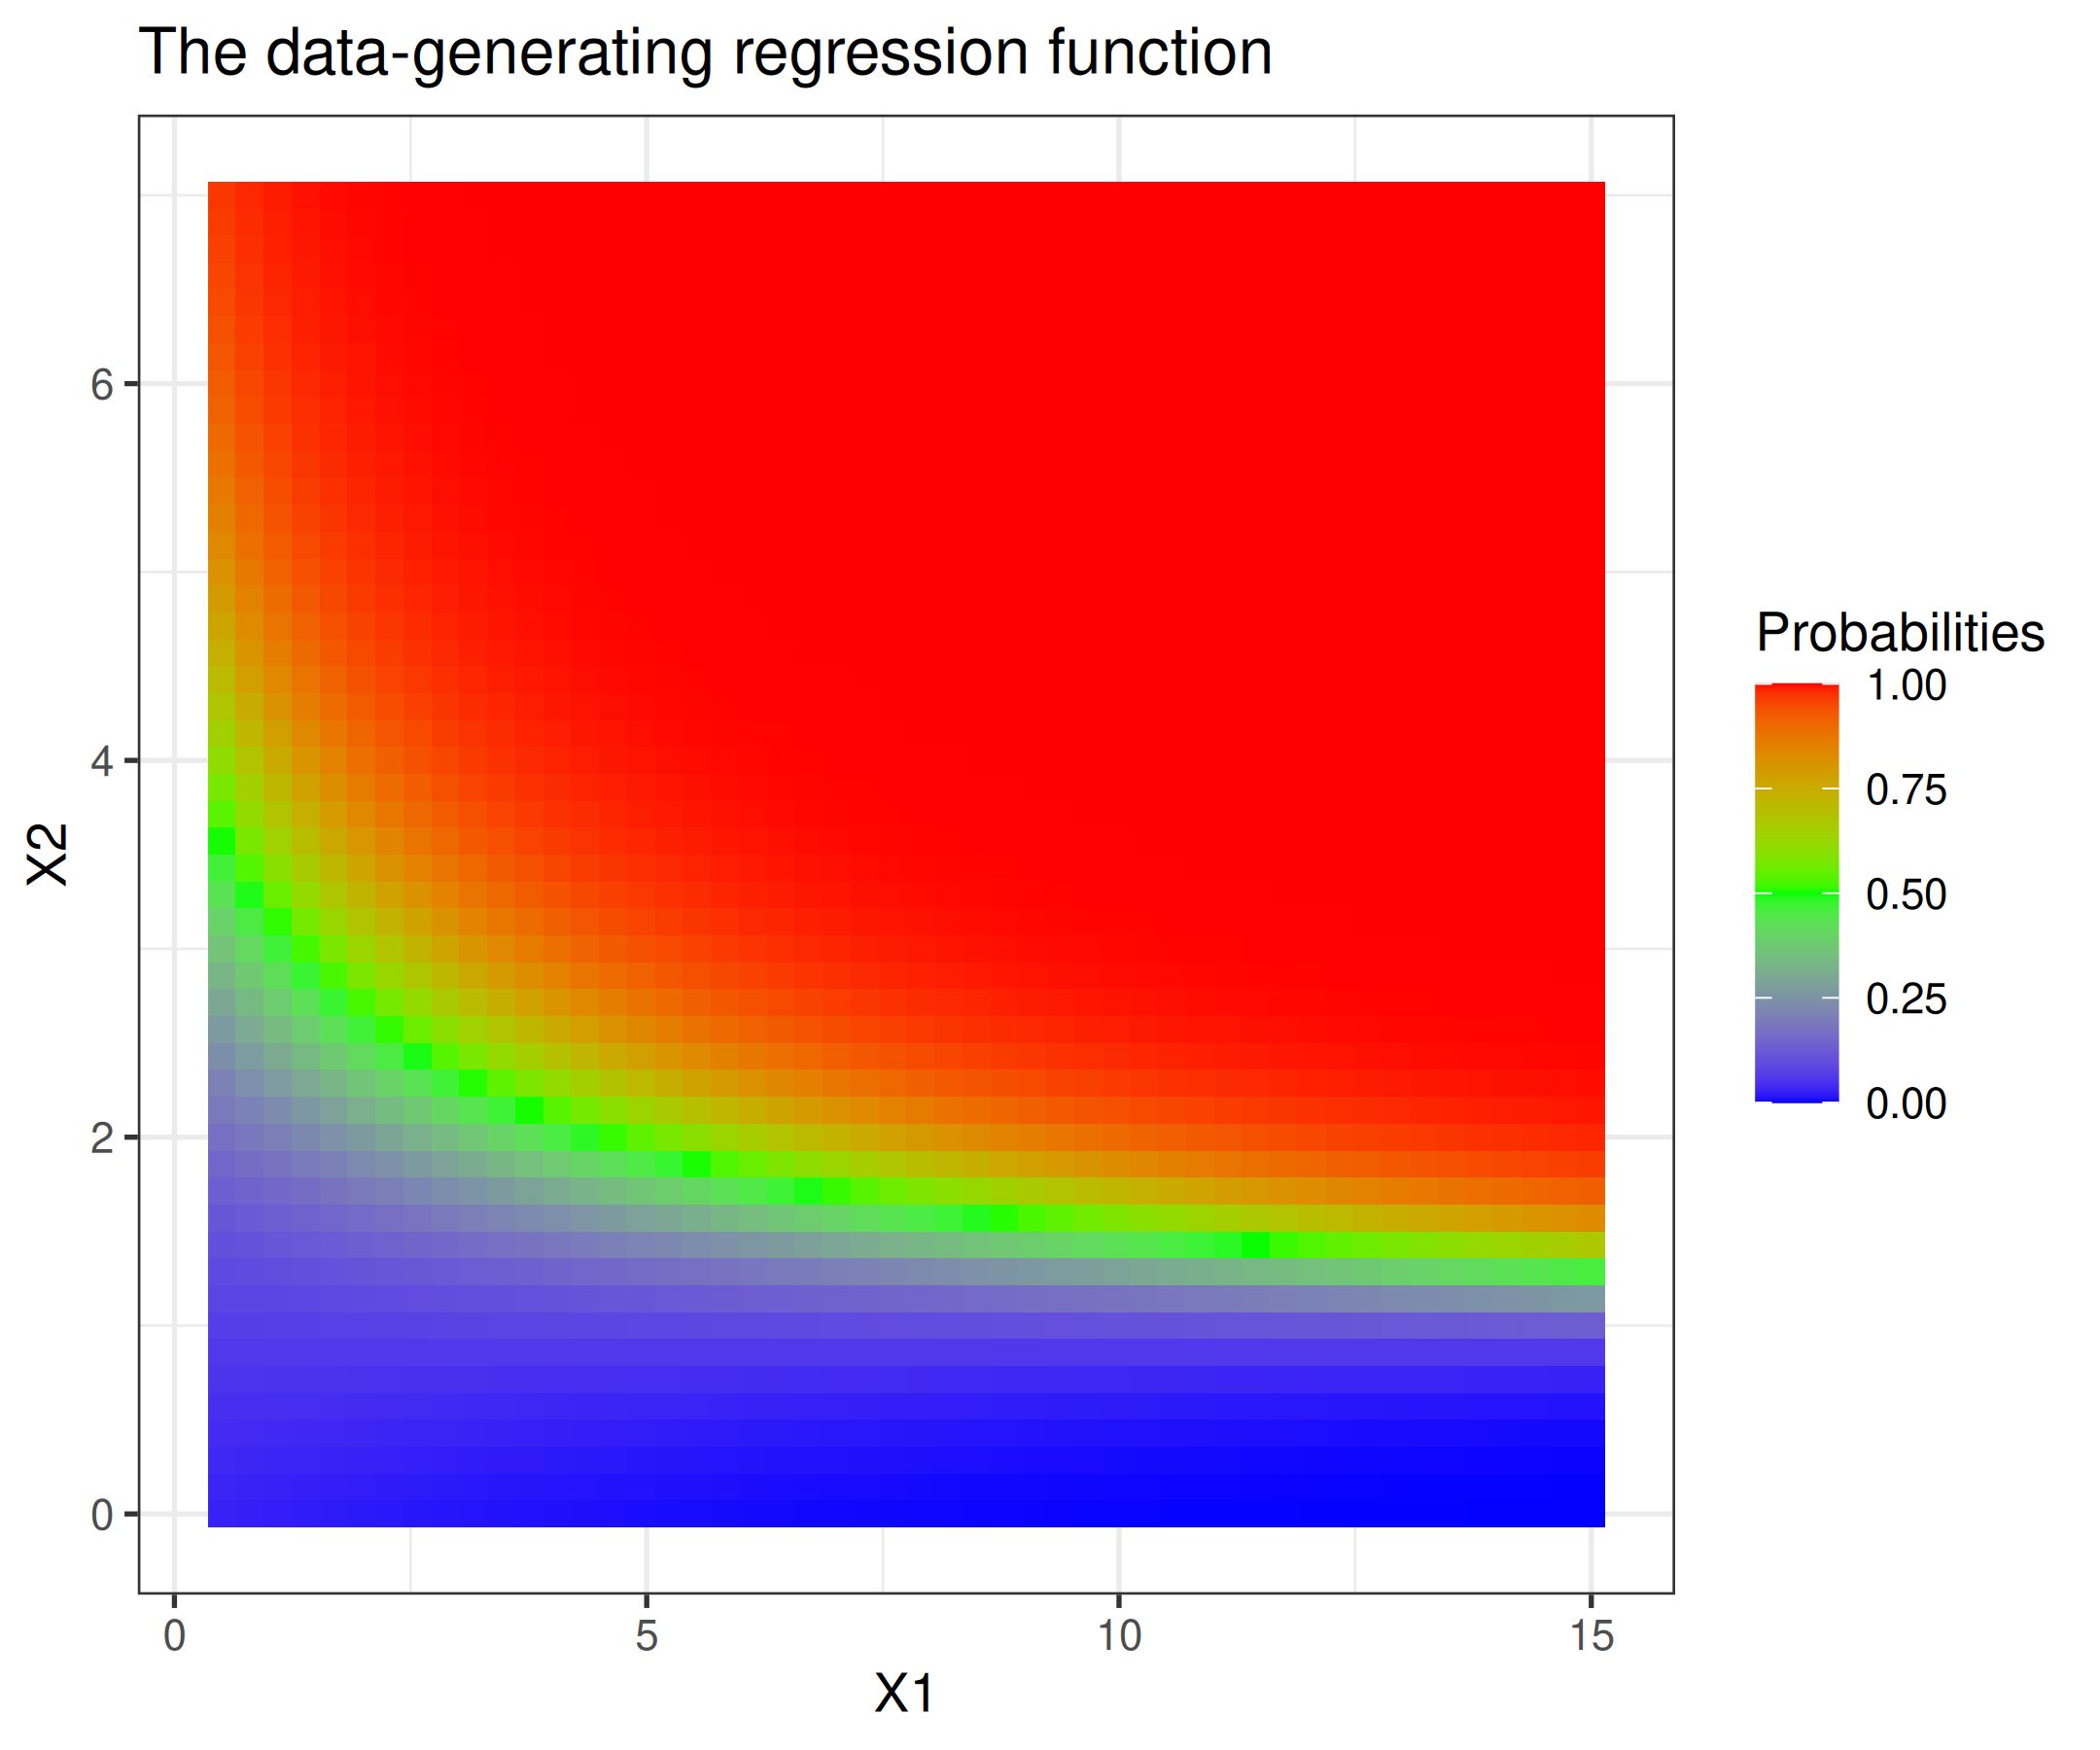
\includegraphics[width=0.8\textwidth]{figures/trueplot.png}
    \caption{The data-generating regression plotted as a heat map}
    \label{fig:trueplot}
\end{figure}
The regression is captured by the logistic regression model with interaction terms. We will use the following library of learning algorithms as an illustrative example:
\begin{enumerate}
    \item Intercept only logistic regression: $E[Y \mid X_1, X_2] = \expit(\beta_0)$
    \item Logistic regression with main effects: $E[Y \mid X_1, X_2] = \expit(\beta_0 + \beta_1 X_1 + \beta_2 X_2)$
    \item XGBoost with hyperparameters: \texttt{max\_depth=3, eta=0.3,\\ n\_rounds=100, objective='binary:logistic', booster='dart', nthread=5}
\end{enumerate}
As we have have been able to plot the data-generating regression, we can also visualize the predictions of the learning algorithms in the library similarly. In figure \ref{fig:predictpar} we visualize the predictions of the main effects logistic regression and XGBoost fitted using 1000 observations sampled from the distribution. 
\begin{figure}
    \centering
    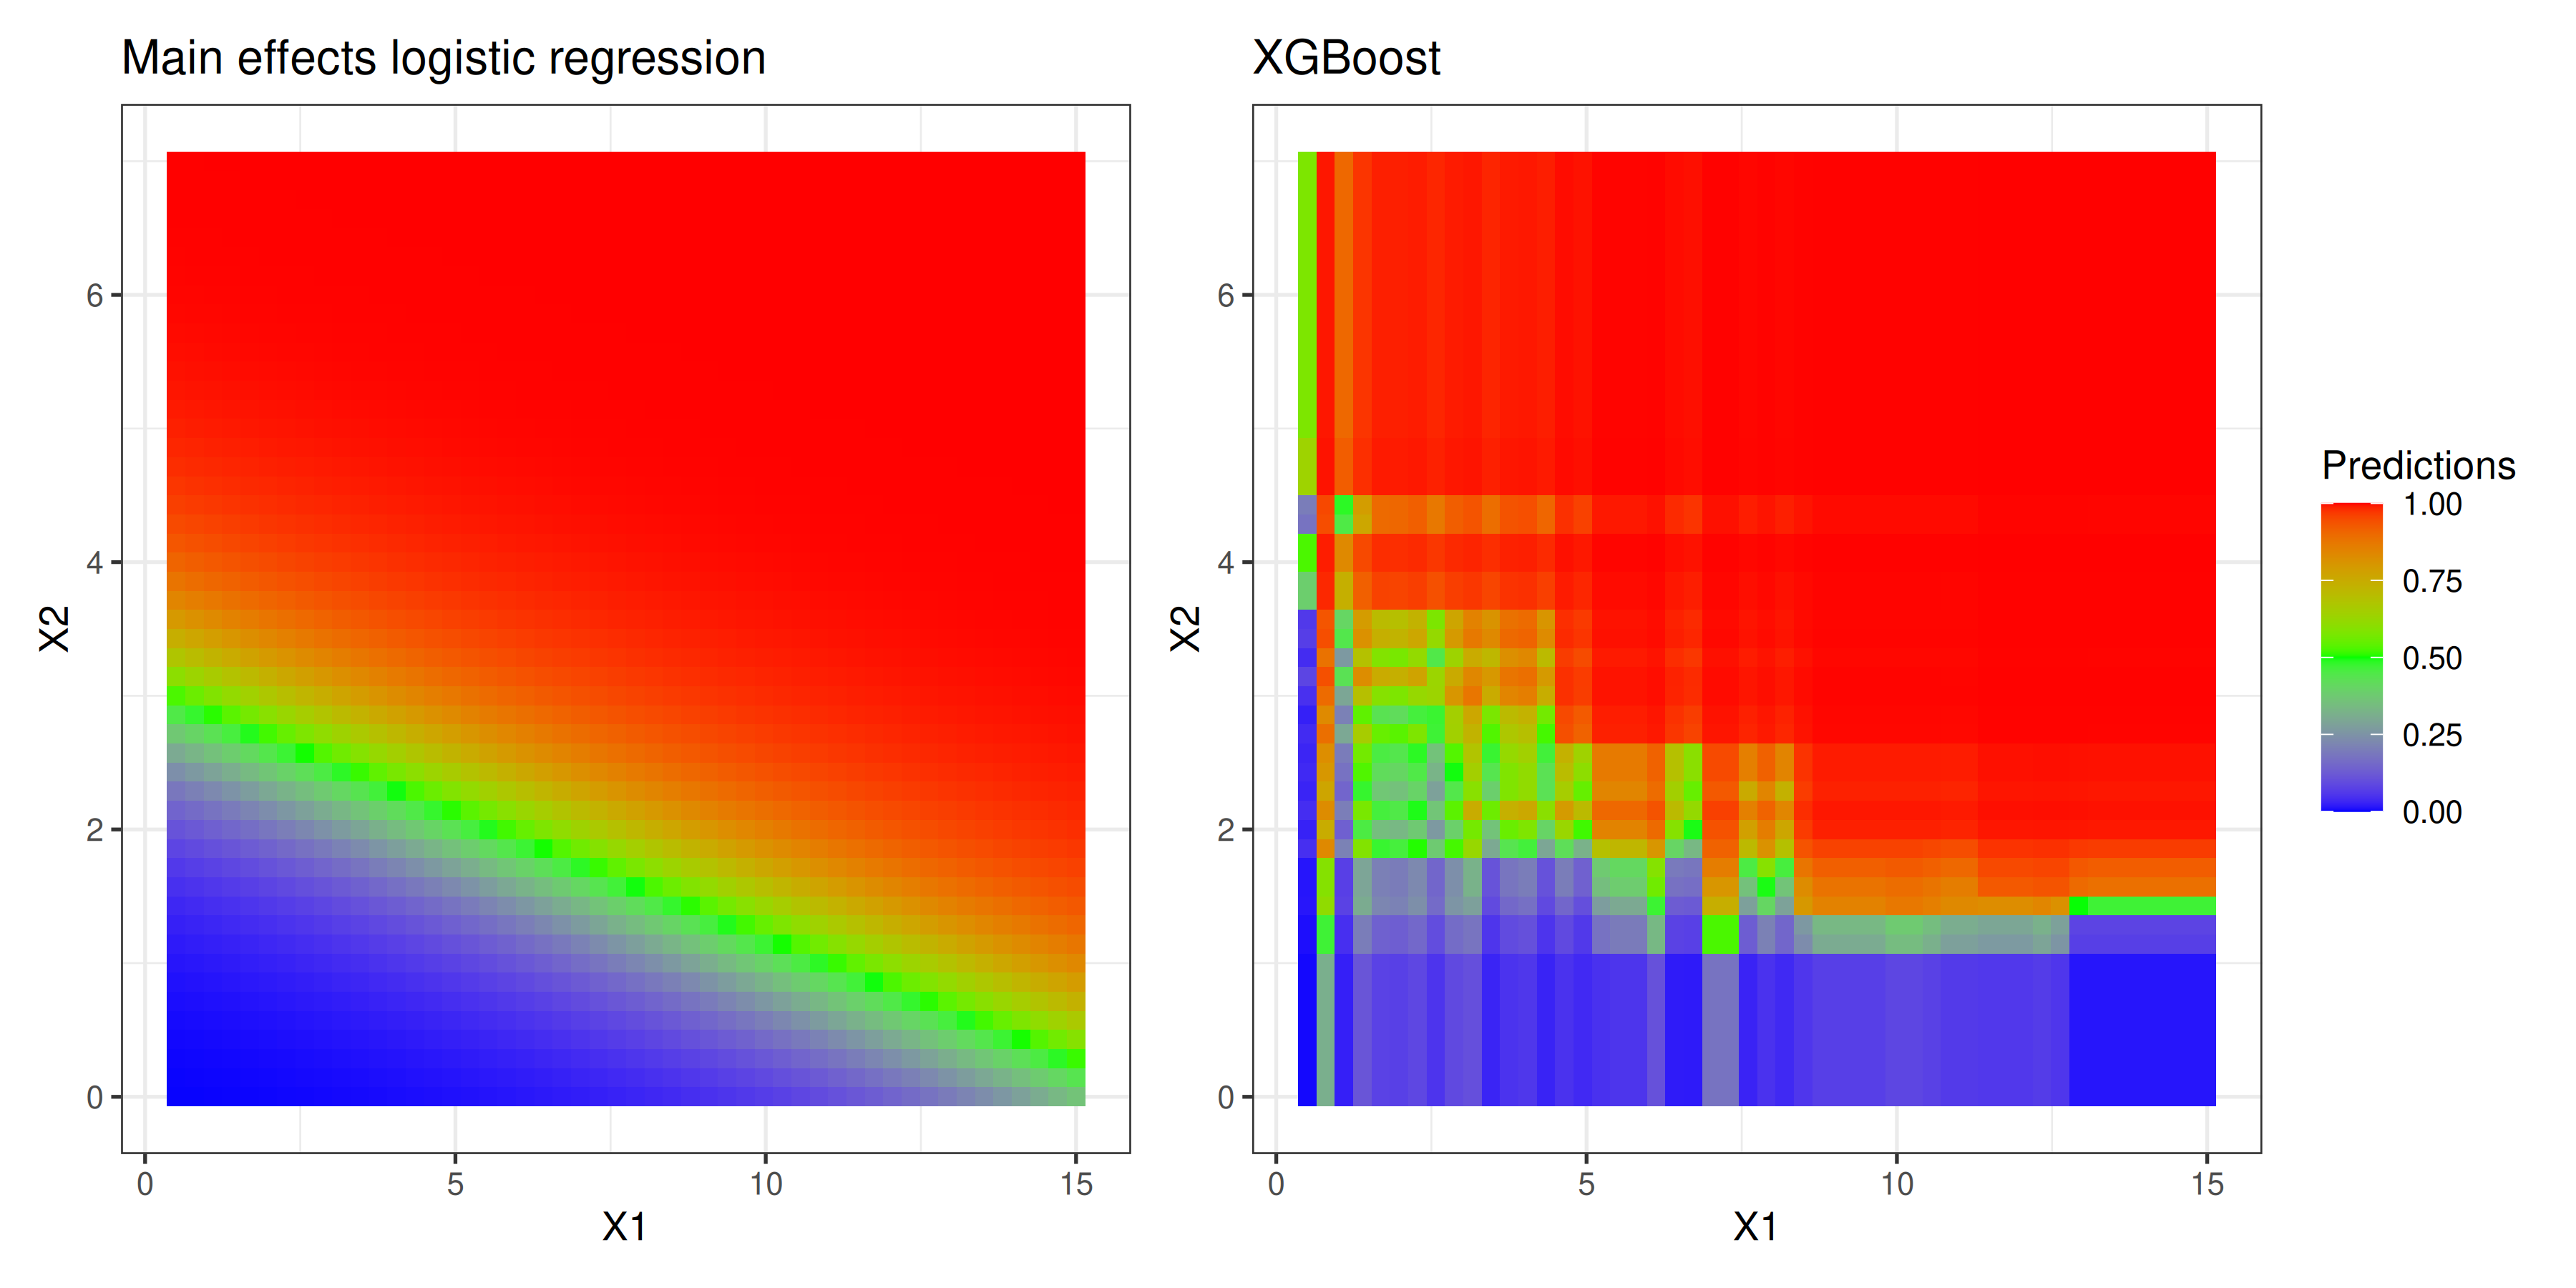
\includegraphics[width=\textwidth]{figures/predictpar.png}
    \caption{The predictions of the main effects logistic regression and XGBoost plotted as a heat map}
    \label{fig:predictpar}
\end{figure}
The plot for the intercept only logistic regression is omitted, as its appearance is as one would expect -- the plot is simply an orange square.

From figure \ref{fig:predictpar} we can observe a clear difference in the predicted probabilities between the logistic regression and the tree-based XGBoost. The main effects logistic regression is a parametric model that assumes that the regression function is a smooth transformation of the linear predictor $ X\beta $. XGBoost, in contrast, is made up of decision trees, which explains the patchwork pattern in its prediction plot. For small samples and as we will see in the simulations, XGBoost has a high risk in comparison to the main effects logistic regression despite the fact that it is misspecified. However, XGBoost becomes increasingly better at approximating the true regression when the number of observations becomes large as seen in figure \ref{fig:xgboost10k}. By applying a super learning algorithm to the library, we will see that the cross-validation selector is able to qualitatively assess and select the best learning algorithm to apply given the amount of data at hand. For example the cross-validation selector might select the main effects logistic regression in the beginning with few training samples, but as the predictions of XGBoost become more stable with more samples, the selector is likely to shift its preference towards XGBoost.  
\begin{figure}[H]
    \centering
    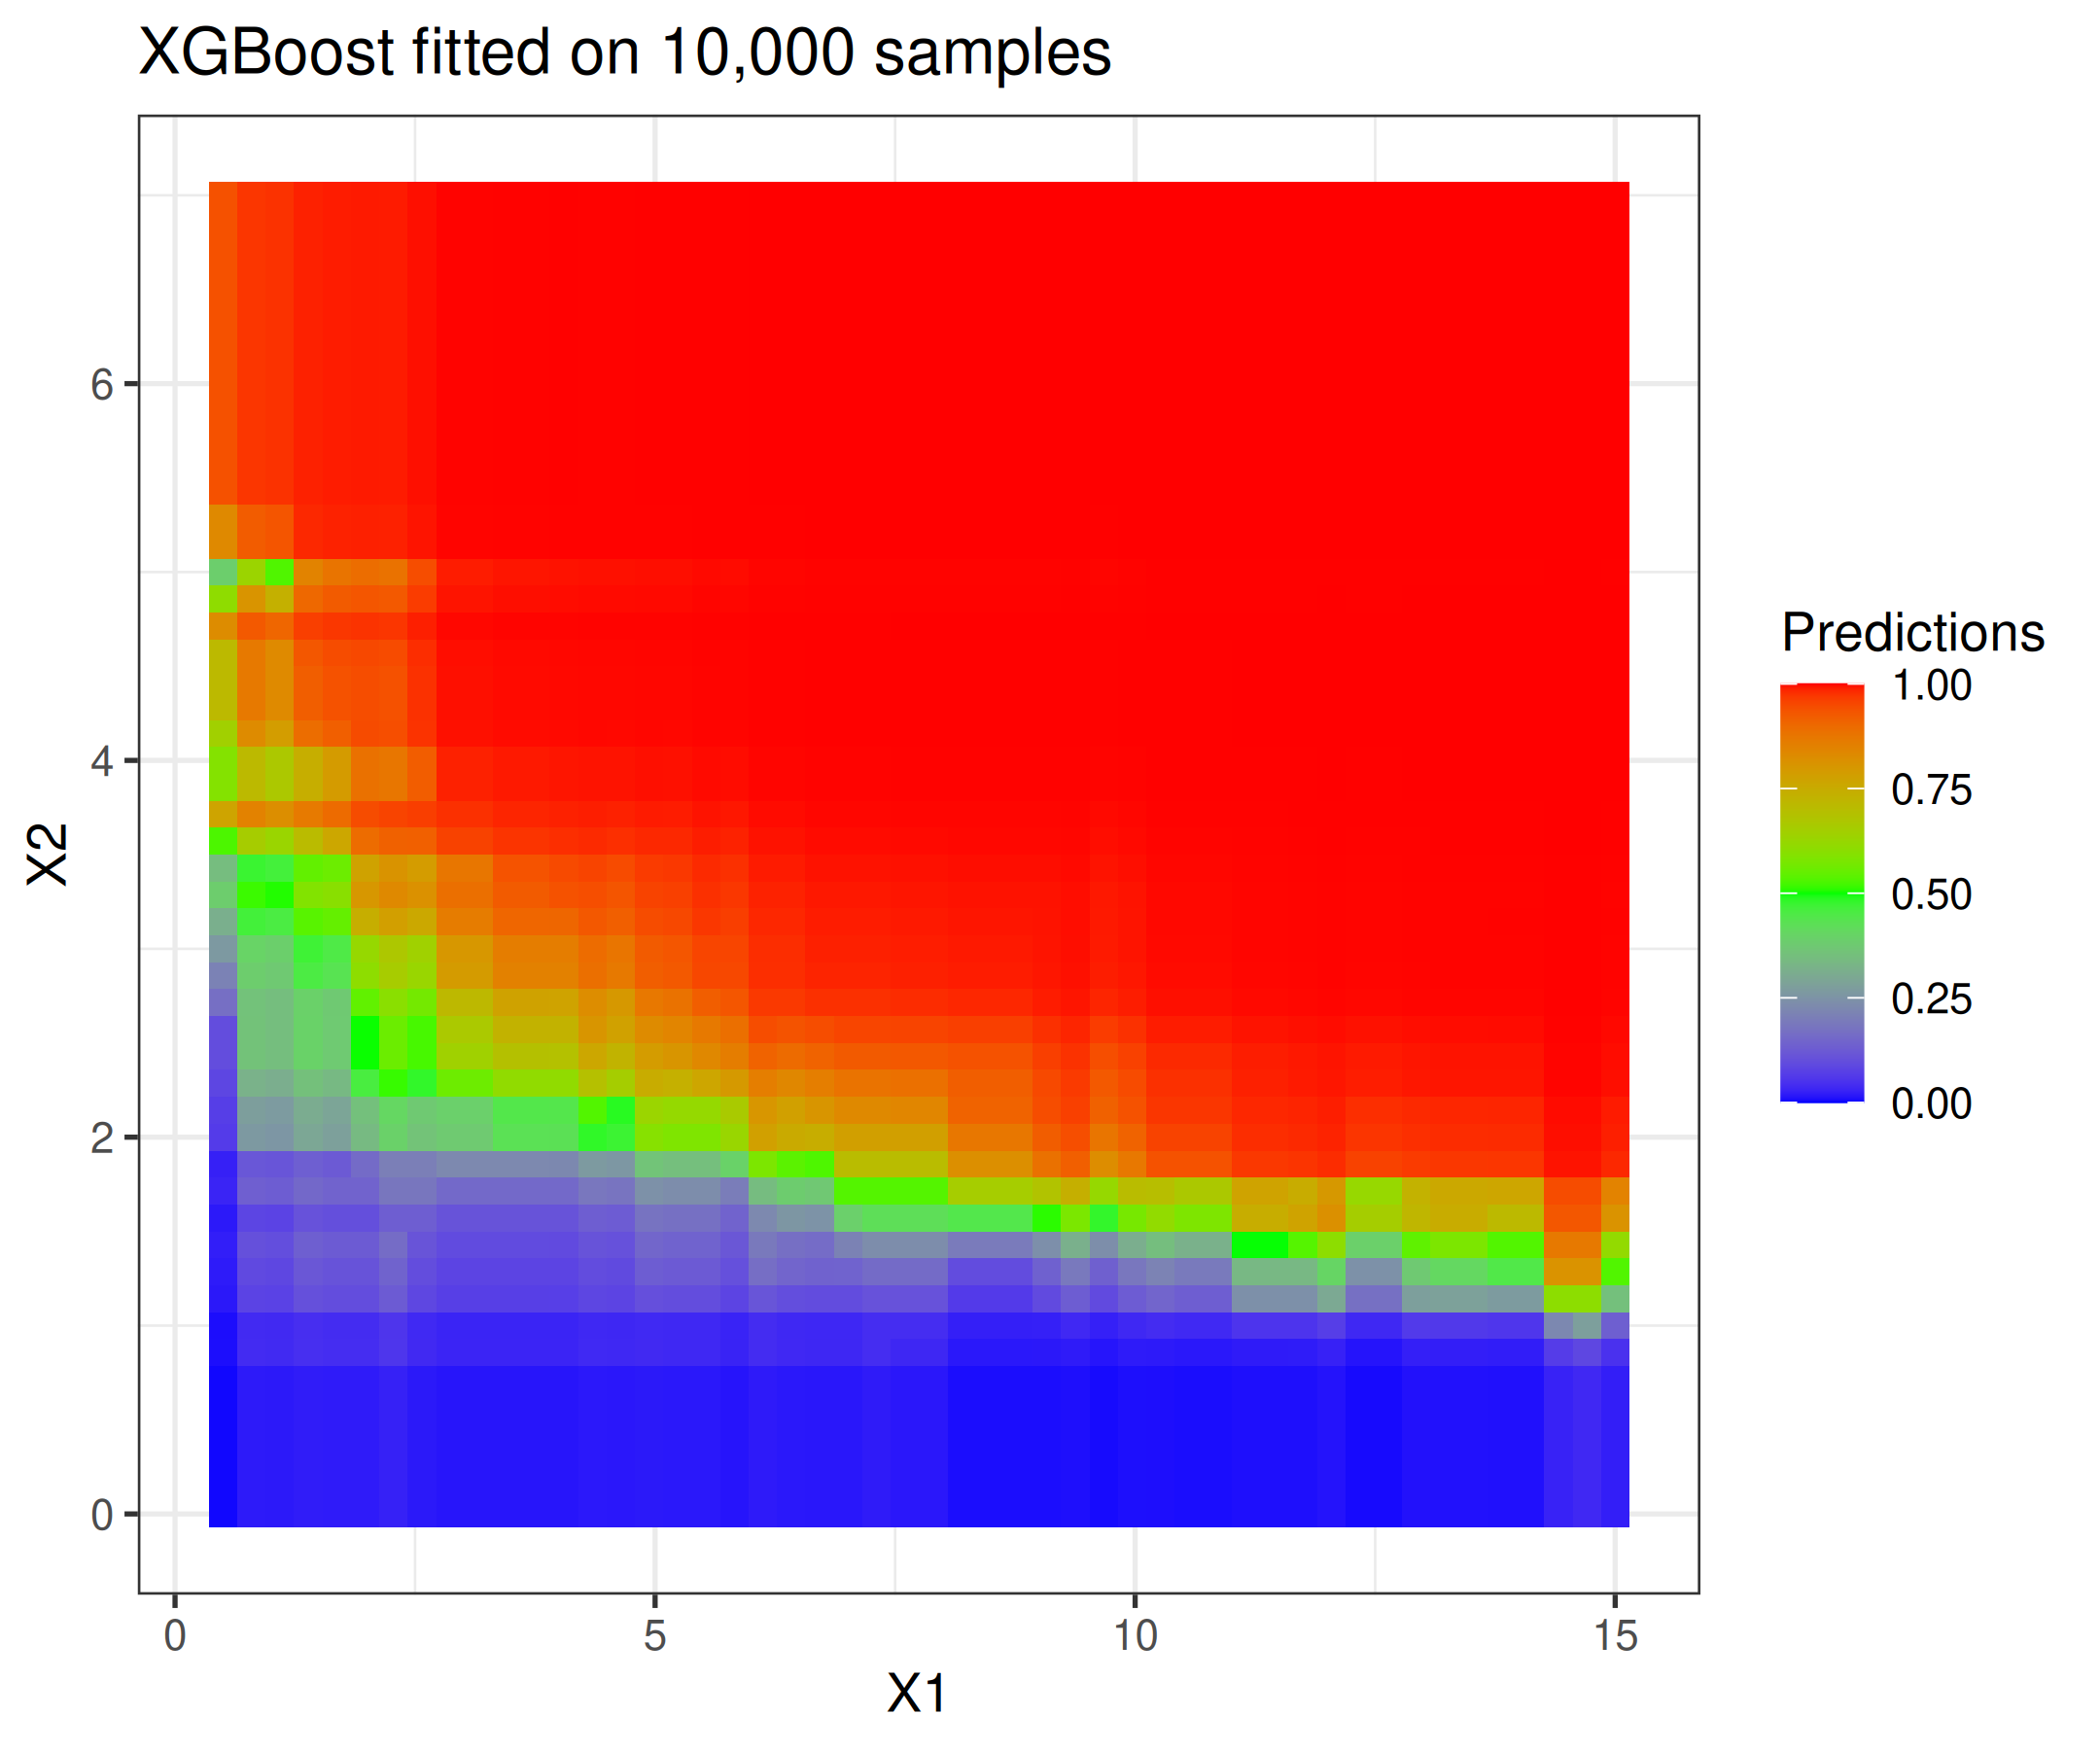
\includegraphics[width=0.7\textwidth]{figures/xgboost10k.png}
    \caption{XGBoost becoming better at approximating the true regression as the sample size increases}
    \label{fig:xgboost10k}
\end{figure}
In our setup, we will consider a discrete super learner that uses 10-fold cross validation and the internal loss function will be the quadratic loss. The performance of the discrete super learner will be compared to each individual learner in the library. We show that
\begin{enumerate}
    \item As the sample size increases, the  discrete super learner achieves the minimum risk 
    \item For a single new observation, the prediction of the discrete super learner on the outcome has the lowest variance
\end{enumerate}
\subsection{Simulation results for the discrete super learner}
\begin{figure}[H]
    \centering
    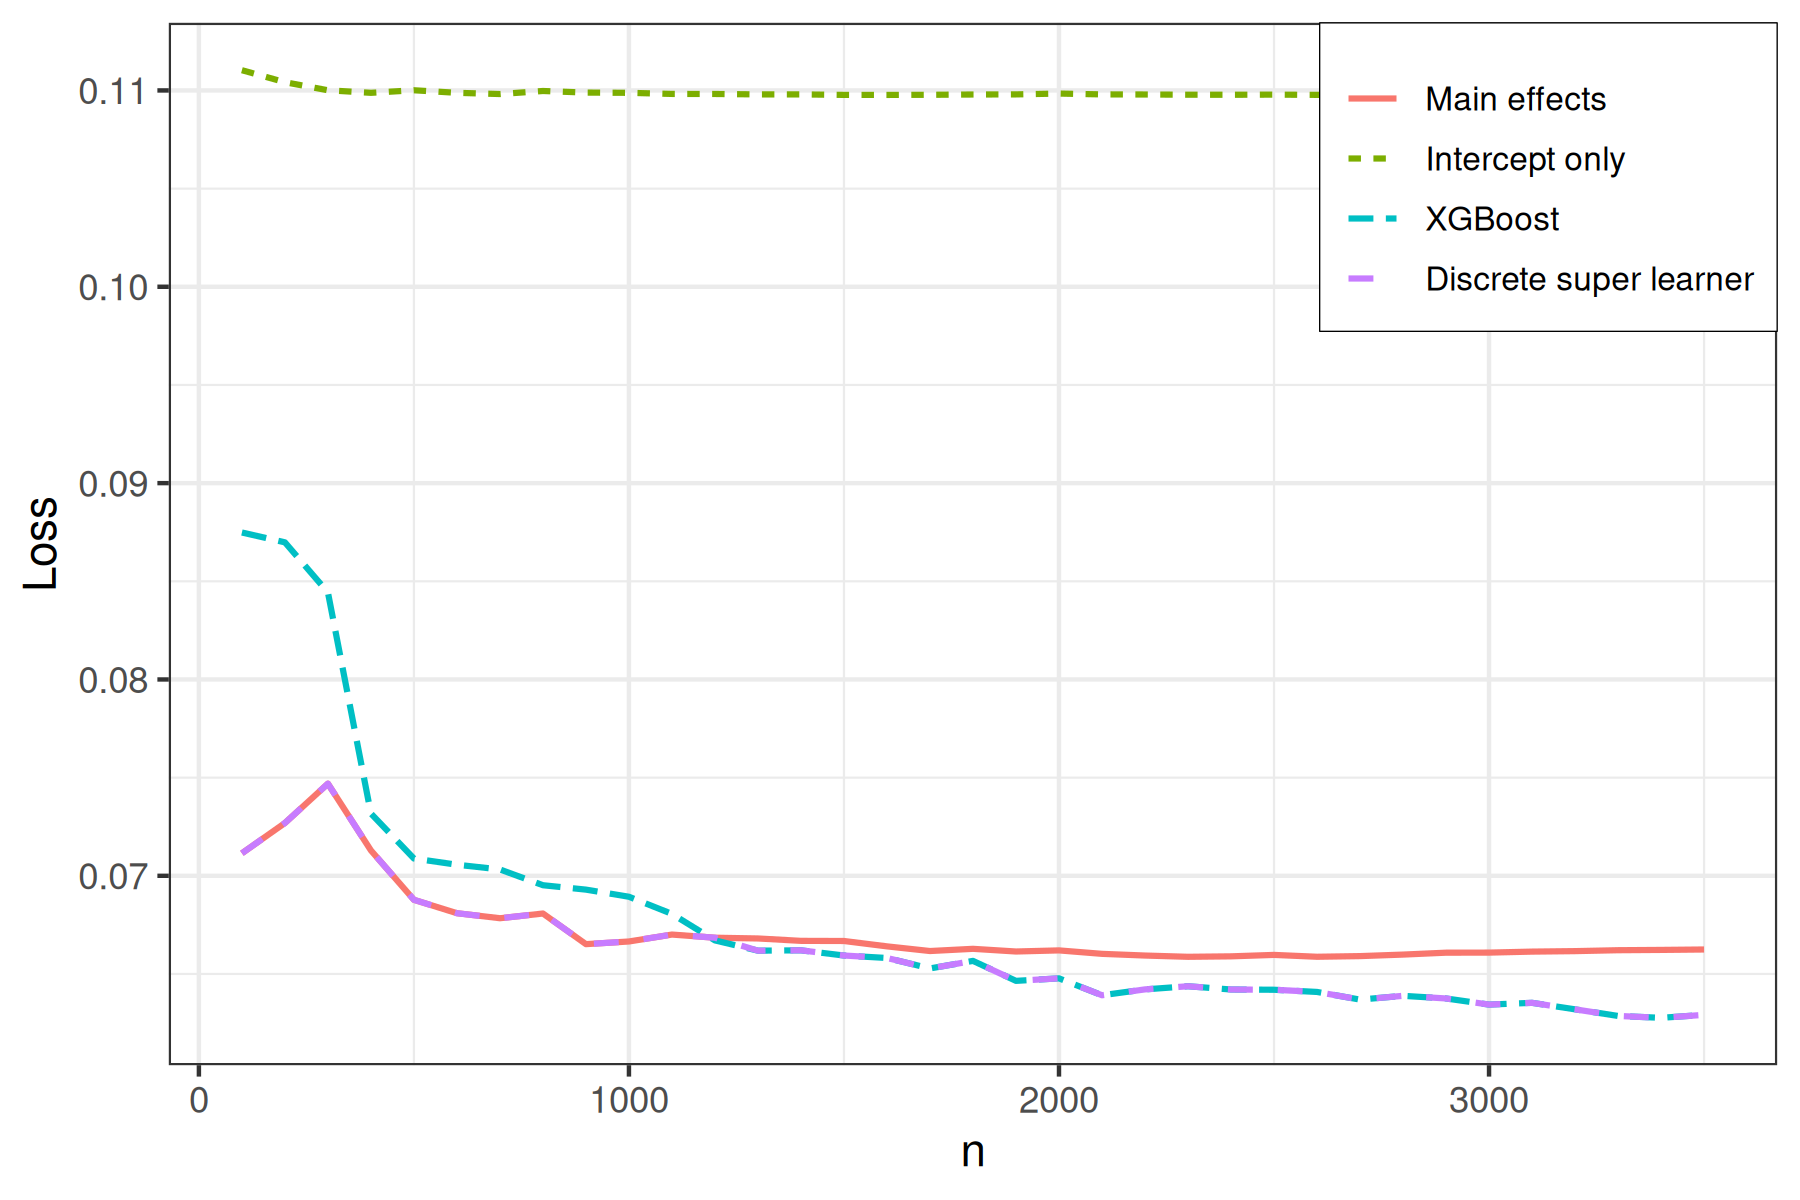
\includegraphics[width=\textwidth]{figures/dsl_loss.png}
    \caption{The risk of the discrete super learner compared to other learners. $ N = 3500 $} 
    \label{fig:loss_min_of_both}
\end{figure}


\begin{figure}[H]
    \centering
    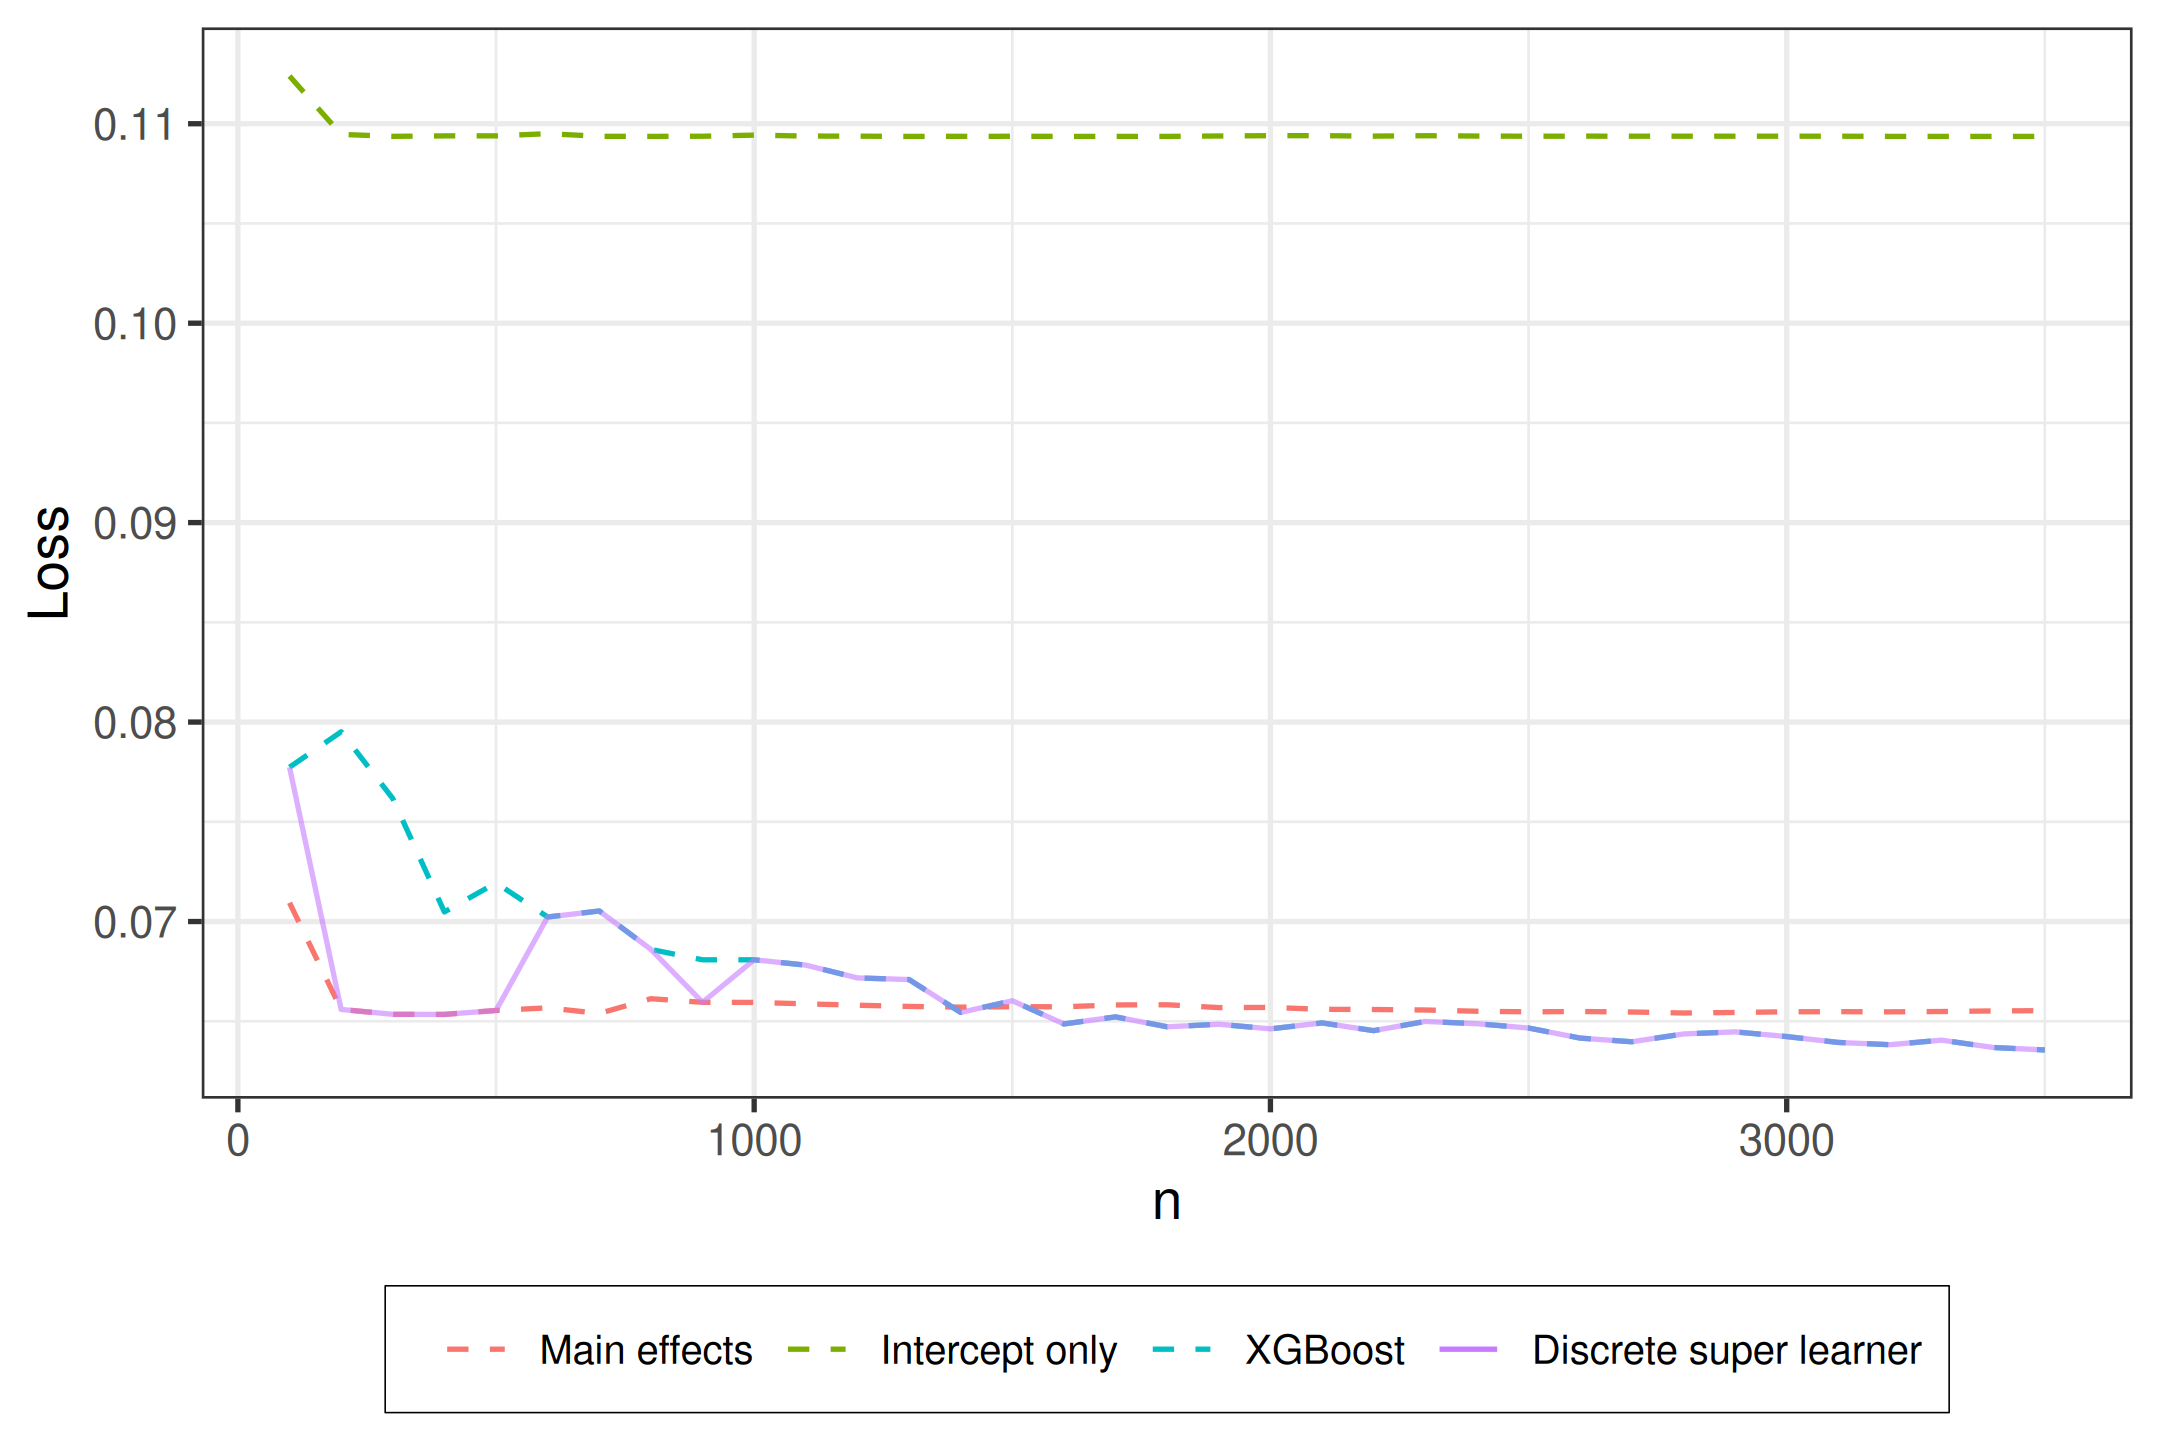
\includegraphics[width=\textwidth]{figures/dsl_loss_jumps.png}
    \caption{The risk of the discrete super learner compared to other learners. $ N = 3500 $}
    \label{fig:loss_jumps}
\end{figure}

\begin{figure}[H]
    \centering
    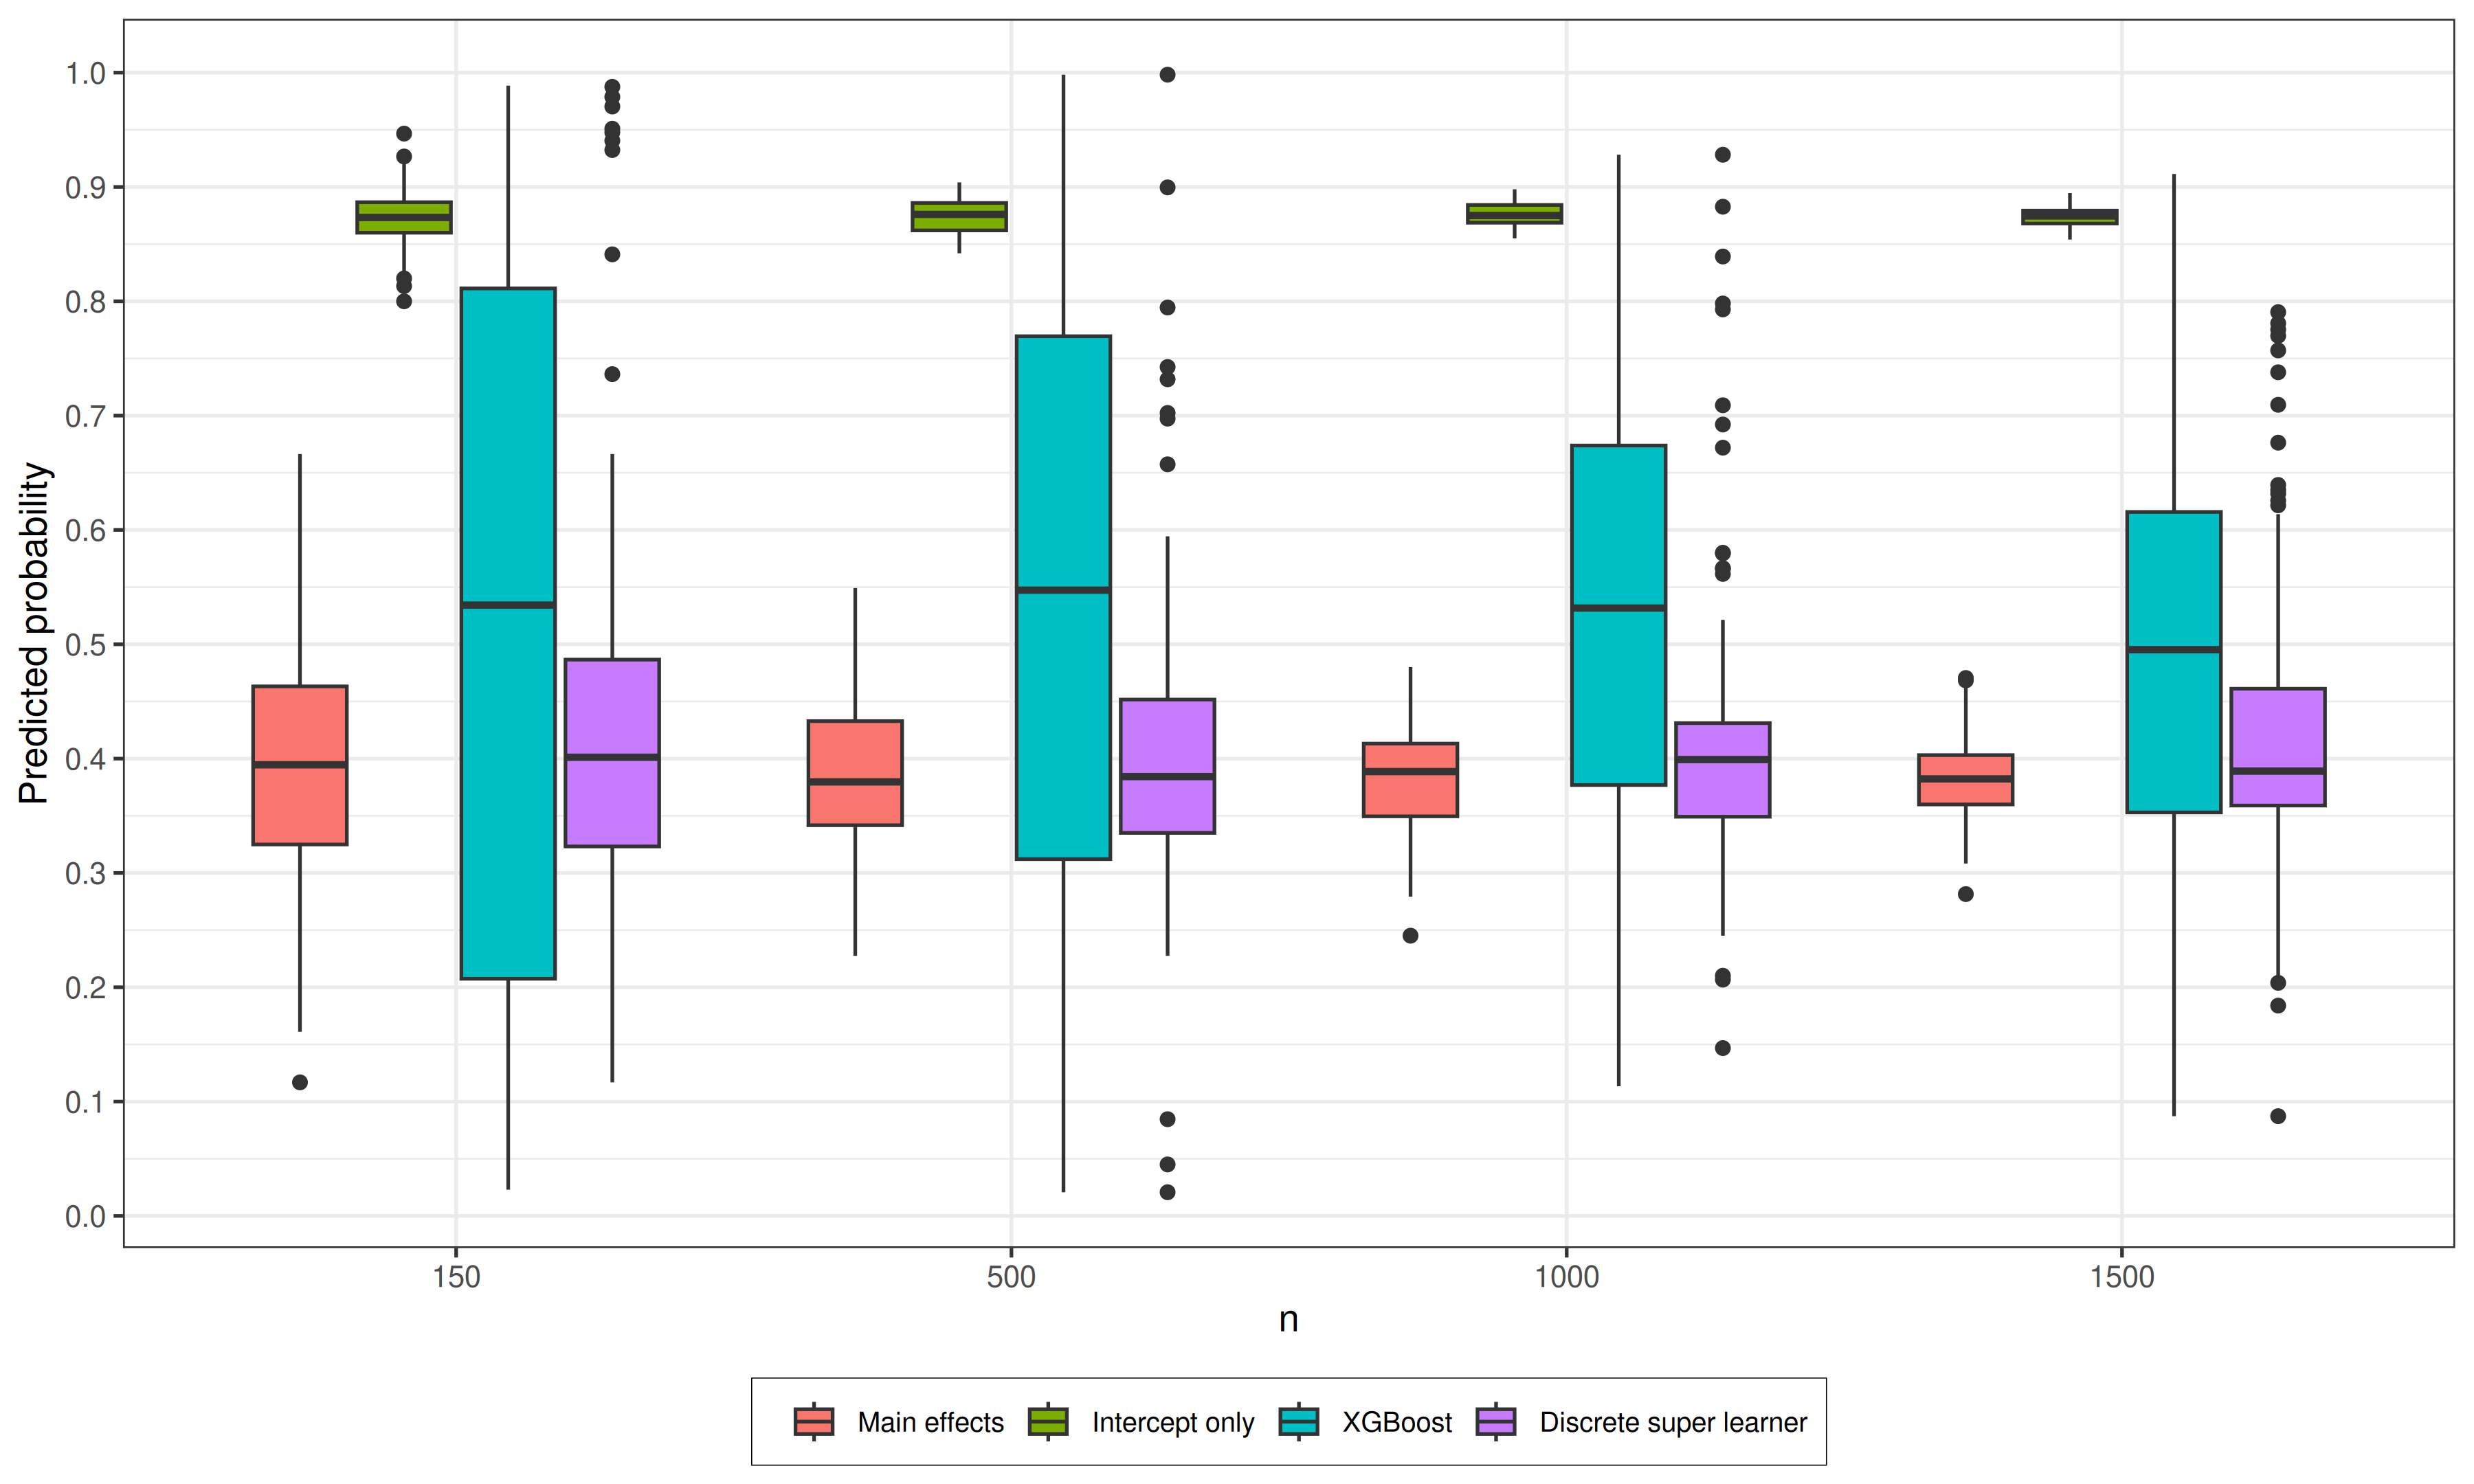
\includegraphics[width=\textwidth]{figures/learner_vars.png}
    \caption{Variances of learner predictions for a single observation, each trained on $n $ samples and evaluated $ K = 1000 $ times on a single observation}
    \label{fig:pred_probs_boxplot}
\end{figure}

\subsection{Discussion of results}
Figures \ref{fig:loss_min_of_both} and \ref{fig:loss_jumps} illustrate how the discrete super learner performs in comparison to the learners in terms of loss over number of training samples. The plots are generated for two runs where the model is fitted on $ n = 100, 200, \dots , 3500 $ observations, as indicated on the $ x $-axis, then the empirical risk is calculated by evaluating each fitted learner on a fixed test sample of size of $ 5000 $. The test data is sampled from the data-generating distribution.  

The first run perfectly illustrates how the discrete super learner is able to achieve the minimum risk. For small training sample sizes, the machine learning method XGBoost has a higher risk than the main effects logistic regression, and it is therefore more desirable for the discrete super learner to choose logistic regression despite the fact that it is misspecified. The discrete super learner consequently achieves the same risk as the logistic regression in the beginning, but for $ n > 1200 $ the risk of the discrete super learner becomes less than the logistic regression. Here XGBoost begins to achieve a lower risk than the misspecified logistic regression, and so the discrete super learner chooses XGBoost instead. 

The second run shows that the discrete super learner might be unable to determine the learner with the lowest risk when the training sample size is small, which results in it moving in a zig-zag pattern between two learners that have quite similar risks. However, we see that the discrete super learner eventually chooses XGBoost as the training sample size becomes larger.  

Figure \ref{fig:pred_probs_boxplot} shows the variance of the predictions of each learner for a single observation, whose true probability is indicated by the red dashed line. Each learner have been trained $ K = 1000 $ times on $ n = 150, 500, \dots 3000 $ samples and is used to predict $ K $ times after each training. The box plots are created from the $ K $ predictions. 

We observe that the machine learning model, XGBoost, has the highest prediction variance across all training sample sizes. Recall that we only had two covariates, here having 1500 observations limits the range of predictions of our main effects model to be between $ 0.27 $ and $ 0.46 $. Whereas for XGBoost the predictions can vary from below $ 0.1 $ to above $ 0.9 $. While XGBoost is extremely efficient at minimizing loss, its predictions are unreliable unless one has an absurd amount of training data. 

The discrete super learner attempts to b 

\section{Appendix}
\subsection{Proof of lemma \ref{finitesampledecomp}}
\begin{proof}
    We first note that the minimizing property of $ \hat{\la} $ (definition \ref{def:cvselector}) implies that 
    \begin{align}
        E_{\Sn} R( \hat{\la}(P_{n, \Sn}^{0}), P_{n, \Sn}^{1} ) \leq E_{\Sn} R( \tilde{\la}(P_{n, \Sn}^{0}) , P_{n, \Sn}^{1}  ). \label{eq:minizing} 
    \end{align}
   We can write (\ref{eq:minizing}) as  
   \begin{align*}
       E_{\Sn} R( \hat{\la}(P_{n, \Sn}^{0} )&, P_{n, \Sn}^{1}) \leq (1 + 2 \delta) E_{\Sn} R( \tilde{\la}(P_{n, \Sn}^{0}) , P ) \\ 
               &+E_{\Sn} \frac{1}{\sqrt{n_1} } R(\tilde{\la} (P_{n, \Sn}^{0}), (1 + \delta) G_{n,\Sn}^{1} - \delta \sqrt{n_1} P)\\
               &-E_{\Sn} \frac{1}{\sqrt{n_1} } R(\hat{\la}(P_{n, \Sn}^{0}), (1 + \delta) G_{n,\Sn}^{1} + \delta \sqrt{n_1} P)  .
   \end{align*}
  Indeed, by examining the risk in the second term on the right hand we obtain 
  \begin{align*}
      R(\tilde{\la} &(P_{n, \Sn}^{0}), (1 + \delta) G_{n,\Sn}^{1} - \delta \sqrt{n_1} P)\\
                    &= (1 + \delta) R(\tilde{\la} (P_{n, \Sn}^{0}), G_{n,\Sn}^{1}) - \delta \sqrt{n_1} R(\tilde{\la} (P_{n, \Sn}^{0}), P) \\ 
                    &= (1 + \delta) \left[\sqrt{n_1} R(\tilde{\la} (P_{n, \Sn}^{0}), P_{n,\Sn}^{1}) - \sqrt{n_1} R(\tilde{\la} (P_{n, \Sn}^{0}), P)\right] - \delta \sqrt{n_1} R(\tilde{\la} (P_{n, \Sn}^{0}), P)\\ 
                    &= (1 + \delta) \sqrt{n_1} R(\tilde{\la} (P_{n, \Sn}^{0}), P_{n,\Sn}^{1}) - (1 + 2\delta)\sqrt{n_1}   R(\tilde{\la} (P_{n, \Sn}^{0}), P).
  \end{align*}
  And for the third term 
  \begin{align*}
     R&(\hat{\la}(P_{n, \Sn}^{0}), (1 + \delta) G_{n,\Sn}^{1} + \delta \sqrt{n_1} P)\\
       &= (1 + \delta) R(\hat{\la} (P_{n, \Sn}^{0}), G_{n,\Sn}^{1}) + \delta \sqrt{n_1} R(\hat{\la} (P_{n, \Sn}^{0}), P) \\ 
       &= (1 + \delta) \left[\sqrt{n_1} R(\hat{\la} (P_{n, \Sn}^{0}), P_{n,\Sn}^{1}) - \sqrt{n_1} R(\hat{\la} (P_{n, \Sn}^{0}), P)\right] + \delta \sqrt{n_1} R(\hat{\la} (P_{n, \Sn}^{0}), P)\\ 
       &=(1 + \delta) \sqrt{n_1} R(\hat{\la} (P_{n, \Sn}^{0}), P_{n,\Sn}^{1}) - \sqrt{n_1}   R(\hat{\la} (P_{n, \Sn}^{0}), P).
  \end{align*}
  The $ \sqrt{n_1} $ in each term will disappear after we multiply with $ \frac{1}{\sqrt{n_1}} $. We now add the first and second term on the right hand side 
  \begin{align*}
      &(1 + 2 \delta) E_{\Sn} R( \tilde{\la}(P_{n, \Sn}^{0}) , P ) +E_{\Sn} \frac{1}{\sqrt{n_1} } R(\tilde{\la} (P_{n, \Sn}^{0}), (1 + \delta) G_{n,\Sn}^{1} - \delta \sqrt{n_1} P)\\ 
      &= (1 + 2 \delta) E_{\Sn} R( \tilde{\la}(P_{n, \Sn}^{0}) , P ) + E_{\Sn} \left[(1 + \delta) R(\tilde{\la} (P_{n, \Sn}^{0}), P_{n,\Sn}^{1}) - (1 + 2\delta)R(\tilde{\la} (P_{n, \Sn}^{0}), P) \right]\\
      &=(1 + \delta) E_{\Sn} R(\tilde{\la} (P_{n, \Sn}^{0}), P_{n,\Sn}^{1}).
  \end{align*}
Now by combining all terms on the right hand side we get
\begin{align*}
    &(1 + \delta) E_{\Sn} R(\tilde{\la} (P_{n, \Sn}^{0}), P_{n,\Sn}^{1})\\
    &-E_{\Sn} \frac{1}{\sqrt{n_1} } \left[ (1 + \delta) \sqrt{n_1} R(\hat{\la} (P_{n, \Sn}^{0}), P_{n,\Sn}^{1}) - \sqrt{n_1}   R(\hat{\la} (P_{n, \Sn}^{0}), P) \right] \\
    &= (1 + \delta) E_{\Sn} R(\tilde{\la} (P_{n, \Sn}^{0}), P_{n,\Sn}^{1})- (1 + \delta)E_{\Sn}R(\hat{\la} (P_{n, \Sn}^{0}), P_{n,\Sn}^{1})+ E_{\Sn} R(\hat{\la} (P_{n, \Sn}^{0}), P)
\end{align*}
By the minimizing property the difference between the second and first term must be positive. Since we are adding a positive number to $ E_{\Sn} R(\hat{\la} (P_{n, \Sn}^{0}), P) $, it follows that it must be less than whatever is on the right. In the final lemma we replace $ \hat{\la}  $ and $ \tilde{\la}  $ by the maximum over $ \lib $.  
  
\end{proof}
\printbibliography
\end{document}
